\documentclass[11pt]{article}
\usepackage[a4paper,margin=1in]{geometry}
\usepackage{microtype}
\usepackage{parskip}
\usepackage{amsmath}
\usepackage{amssymb}

\usepackage{graphicx}
\usepackage{subcaption}
\usepackage{booktabs}
\usepackage{array}
\usepackage{tikz}

\usepackage{framed}


\usepackage[colorlinks=true,
            linkcolor=black,
            citecolor=black,
            urlcolor=blue!60!black]{hyperref}

%% SUGGESTION: The repository is named "SPHINCS-Parameters" but this title says "SHRINCS".
%% Decide which name is canonical and use it consistently throughout the document.
%% (If "SHRINCS" is intentional — the hybrid construction's own name — consider a short
%% footnote on first mention to disambiguate it from SPHINCS+/SLH-DSA.)
\title{SHRINCS Stateless Parameter Search Methodology}
\date{\today}

\begin{document}

\maketitle

\tableofcontents
\vspace{1em}

\section{Introduction} \label{sec:introduction}
In the case of Bitcoin, hash-based signature schemes are the most compatible among all quantum-resistant signature algorithms. Still, the smallest stateless hash-based signature proposed by NIST (SLH-DSA-128s) is \emph{7,856} bytes \cite{nist}, which is more than $100\times$ larger than the current Schnorr signature. The question is whether we can have something smaller and more practical without significant deviation from the standard.

SHRINCS \cite{delving-post} proposes a hybrid signature consisting of a stateful and a stateless part, with signature size ranging from \emph{324} bytes (stateful) to \emph{X} bytes (stateless). This document attempts to answer the question of what the value of \emph{X} might be while keeping other signature metrics (KeyGen, SigGen, SigVer, etc.) practical.

In this document, we present the methodology for searching parameters of SLH-DSA-compatible signatures: how changes in the hyper-tree structure and other parameters affect the signature metrics. As mentioned above, we deliberately stay within very conservative bounds and avoid any changes to the signature sub-algorithms in order to keep the construction as compatible as possible with the SLH-DSA standard.

\textit{Along the way, we will occasionally reference promising proposals such as hyper-tree pruning \cite{conduition-blog} and the +C compression technique \cite{mike-paper}, which allow for even better shrinking results. Although some of them can be considered partially compatible, we do not rely on them in the evaluation framework. We still think it is useful to outline the potential of such techniques and to let the reader tweak the parameters accordingly.}

The main contributions of this report are (1) a sweep script, (2) the filtering pipeline, and (3) a recommended candidate tuple.
\section{Parameters Description}

\subsection{Initial Bounds}
As mentioned in the introduction, our objective is to find parameters that make the signature ``better'' than SLH-DSA. Before we can do so, we have to fix the strict boundaries that we will not cross:
\begin{enumerate}
    \item We obviously do not want a signature larger than SLH-DSA - otherwise, why bother in the first place?
    \item For Bitcoin, we require at least a 128-bit security level. None of the parameters we select may degrade security below this floor.
    \item At least $q_{s} = 2^{40}$ supported signatures. SLH-DSA-128s defines the maximum number of signatures as $q_{s} = 2^{64}$, which is generous. For Bitcoin, we assume that $q_{s} = 2^{40}$ is a practical compromise, comfortably covering the foreseeable needs of on-chain operations and the Lightning Network.
    \item Sub-algorithms, hash, and addressing functions remain unchanged.
\end{enumerate}

\subsection{SLH-DSA Parameters}
SLH-DSA uses a hyper-tree of eXtended Merkle Signature Schemes (XMSS) to authenticate the underlying one-time and few-time signature keys. We formally parameterize each candidate configuration using the tuple $(h, d, k, a, w)$, where each variable controls a distinct geometric trade-off within the overall structure.

\paragraph{Hyper-Tree Geometry ($h$ and $d$).}
The hyper-tree configuration determines the capacity and layer-traversal costs of the signature scheme.
\begin{itemize}
    \item $h$ is the total height of the multi-layered hyper-tree. This dictates the maximum number of few-time signature instances supported at the base layer, yielding a total capacity of $2^h$ unique leaf nodes.
    \item $d$ is the number of independent tree layers comprising the hyper-tree.
\end{itemize}
To ensure a symmetric construction across all internal boundaries, our search pipeline requires that the total height $h$ be perfectly divisible by the layer count $d$. Consequently, each individual XMSS tree layer has a uniform height $h'$:
\begin{equation*}
    h' = \frac{h}{d}.
\end{equation*}
Adjusting the ratio between $h$ and $d$ governs the balance between signature size and key-generation cost. Reducing the number of layers $d$ shrinks the total number of intermediate public keys and authentication paths in the signature payload, saving valuable bytes. However, this exponentially increases the height $h'$ of each constituent tree, requiring significantly more hash operations to compute the root node during key generation.

\paragraph{Few-Time Signature Layer ($k$ and $a$).}
The lowest layer of the hyper-tree authenticates the Forest of Random Subsets (FORS) few-time signature scheme, which directly signs the message digest.
\begin{itemize}
    \item $k$ is the number of independent, parallel Merkle trees in the FORS layer.
    \item $a$ is the height of each individual FORS tree, so that each constituent tree contains exactly $t = 2^a$ leaves.
\end{itemize}

Increasing $k$ and $a$ strengthens the scheme against multi-target subset-forgery attacks and allows the structure to support larger capacities safely. However, expanding these dimensions directly increases the byte footprint of the appended authentication paths.

\paragraph{One-Time Signature Base ($w$).}
Internal tree roots are signed using the Winternitz One-Time Signature Plus (WOTS+) scheme. The base parameter $w$ defines the digit representation used to split the message digest during signing. Our framework evaluates candidate configurations across the standard baseline settings $w \in \{16, 32, 256\}$.

Selecting a larger base reduces the number of parallel hash chains $\ell$, which in turn reduces the overall WOTS+ payload size. This spatial efficiency comes at the cost of local compute: larger base parameters require longer hash chains, resulting in higher execution costs during key and signature generation.

We sweep the ranges as follows:
\begin{equation*}
    (h, d, k, a, w) \in \{40, \dots, 50\} \times \{2, \dots, 24\} \times \{2, \dots, 25\} \times \{8, \dots, 20\} \times \{16, 32, 256\}.
\end{equation*}

\textit{The SLH-DSA-128s baseline tuple (63, 7, 14, 12, 16) sits outside this range and is included for comparison}
\section{Search Methodology}

\subsection{Initial Search Conditions}
Searching for the best parameters requires defining the conditions that the chosen parameter set must satisfy. Consequently, those conditions must rely on metrics that depend on the parameters. We use the following:

\begin{itemize}
    \item \textbf{Signature size}: the size of the signature in bytes;
    \item \textbf{Key generation cost}: the number of SHA-256 compressions during the key-generation phase;
    \item \textbf{Signature generation cost}: the number of compressions executed during signing;
    \item \textbf{Signature verification cost}: the number of compressions during verification;
    \item \textbf{Compressions per byte}: the ratio of verification cost to signature size.
\end{itemize}

We choose SLH-DSA-128s as the baseline for the search; this gives us an intuitive way to compare custom parameter sets against the standardized scheme on equal footing.

\subsection{Toolset}
The methodology described here uses a set of SageMath scripts available at \url{https://github.com/BlockstreamResearch/SPHINCS-Parameters}.

\subsection{Sweep Strategy} \label{sec:sweep-strategy}
We start by enumerating all parameter tuples $(h, d, k, a, w)$. Applying the initial bounds (security level, size $\leq$ SLH-DSA, at least $2^{40}$ supported signatures) reduces the search space from \emph{41,328} candidates to \emph{9,258} - a $78\%$ cut. The remaining space is still too large to inspect by hand, so we need additional filters.

We introduce the following filters\footnote{The coefficient for each filter, except the signature size, may be greater than 1 (meaning we accept some regression on that metric in exchange for gains elsewhere).}:

\begin{itemize}
    \item \textbf{Bound on signature size}: $\mathsf{target.size} \leq c_{\text{size}} \cdot \mathsf{std.size}$, where $c_{\text{size}}$ is a size coefficient ($0 \leq c_{\text{size}} \leq 1$).
    \item \textbf{Bound on key-generation cost}: $\mathsf{target.KeyGen} \leq c_{\text{kg}} \cdot \mathsf{std.KeyGen}$, where $c_{\text{kg}} > 0$.
    \item \textbf{Bound on signature-generation cost}: $\mathsf{target.SigGen} \leq c_{\text{sg}} \cdot \mathsf{std.SigGen}$, where $c_{\text{sg}} > 0$.
    \item \textbf{Bound on signature-verification cost}: $\mathsf{target.SigVer} \leq c_{\text{sv}} \cdot \mathsf{std.SigVer}$, where $c_{\text{sv}} > 0$.
    \item \textbf{Bound on the compressions-per-byte ratio}: $\mathsf{target.C/B} \leq c_{\text{cb}} \cdot \mathsf{std.C/B}$, where $c_{\text{cb}} > 0$.
\end{itemize}


\paragraph{Note:}
All verification cost reported in this section are \emph{average-case}: they reflect the expected number of compressions for a uniformly random message.
The \emph{worst-case} verification cost is approximately $1.94\times$ higher and depends solely on the message being signed — it cannot be influenced by the verifier.
We also use an \emph{average-case} signing cost, while the \emph{worst-case} does not significantly increse the number of compressions to generate a signature.
 

These filters can be combined and parameterized in different ways to produce different result sets. Below, we consider several cases to illustrate how the choice of filter parameters affects the resulting candidate set.

\subsubsection{Case 1: Best in Class}
In this case, we find the most efficient signature for a single metric at a time, leaving the other metrics unbounded. The results are shown in Table~\ref{tab:minimal_metric_each}.

\begin{table}[h!]
\small
\raggedright 
\caption{Absolute Global Extremes}
\label{tab:minimal_metric_each}
\resizebox{\textwidth}{!}{%
\begin{tabular}{llrrrrrrrrr}
\toprule
\textbf{Award Category} & \textbf{Tuple $(h, d, k, a, w)$} & \textbf{Size (B)} & \textbf{VS std, \%} & \textbf{KeyGen ($C$)} & \textbf{VS std, $\times$} & \textbf{SigGen ($C$)} & \textbf{VS std, $\times$} & \textbf{SigVer ($C$)} & \textbf{VS std, $\times$} & \textbf{$\rho$ ($C$/B)} \\
\midrule
%---
\texttt{STANDARD} Baseline & $(63, 7, 14, 12, 16)$ & $7856$ & $+0.0\%$ & $2.93 \times 10^5$ & $1.00$ & $2.28 \times 10^6$ & $1.00$ & $2387$ & $1.00$ & $0.30$ \\
%---
Smallest Signature & $(50, 2, 6, 20, 256)$ & \textcolor{green}{$3408$} & \textcolor{green}{$-56.6\%$} & \textcolor{red}{$1.55 \times 10^{11}$} & \textcolor{red}{$5.29 \times 10^5$} & \textcolor{red}{$3.10 \times 10^{11}$} & \textcolor{red}{$1.36 \times 10^5$} & \textcolor{red}{$4953$} & \textcolor{red}{$2.07$} & \textcolor{red}{$1.45$} \\
%---
Fastest Keygen & $(44, 11, 7, 19, 32)$ & \textcolor{red}{$7712$} & \textcolor{red}{$-1.8\%$} & \textcolor{green}{$1.40 \times 10^4$} & \textcolor{green}{$0.05$} & \textcolor{orange}{$1.48 \times 10^7$} & \textcolor{orange}{$6.51$} & \textcolor{orange}{$5052$} & \textcolor{orange}{$2.12$} & \textcolor{orange}{$0.66$} \\
%---
Fastest Signing & $(40, 8, 23, 8, 32)$ & \textcolor{red}{$7424$} & \textcolor{red}{$-5.5\%$} & \textcolor{green}{$2.80 \times 10^4$} & \textcolor{green}{$0.10$} & \textcolor{green}{$2.47 \times 10^5$} & \textcolor{green}{$0.11$} & \textcolor{orange}{$3888$} & \textcolor{orange}{$1.63$} & \textcolor{orange}{$0.52$} \\
%---
Fastest Verification & $(50, 2, 7, 17, 16)$ & \textcolor{green}{$3952$} & \textcolor{green}{$-49.7\%$} & \textcolor{red}{$1.92 \times 10^{10}$} & \textcolor{red}{$6.55 \times 10^4$} & \textcolor{red}{$3.84 \times 10^{10}$} & \textcolor{red}{$1.68 \times 10^4$} & \textcolor{green}{$894$} & \textcolor{green}{$0.37$} & \textcolor{green}{$0.23$} \\
%---
Best Density Ratio (\texorpdfstring{$\rho$}{rho}) & $(50, 2, 23, 15, 16)$ & \textcolor{red}{$7824$} & \textcolor{red}{$-0.4\%$} & \textcolor{red}{$1.92 \times 10^{10}$} & \textcolor{red}{$6.55 \times 10^4$} & \textcolor{red}{$3.84 \times 10^{10}$} & \textcolor{red}{$1.68 \times 10^4$} & \textcolor{green}{$1366$} & \textcolor{green}{$0.57$} & \textcolor{green}{$0.17$} \\
\bottomrule
\end{tabular}%
}
\end{table}


Table~\ref{tab:minimal_metric_each} confirms what one would suspect: each metric can be minimized impressively in isolation, but only at a brutal cost to the others, leaving these parameter sets unusable in practice. We therefore consider a different strategy.

\subsubsection{Case 2: Balanced Metrics}
In the next experiment, we look for ``average'' candidates whose metrics all stay below a uniform threshold $X \cdot \mathsf{std}$ (the filter is applied to every metric, with the exception of the maximum signature size $\leq \mathsf{std}$). By gradually increasing $X$, we obtain the following picture.
\begin{figure}[h!]
    \centering
    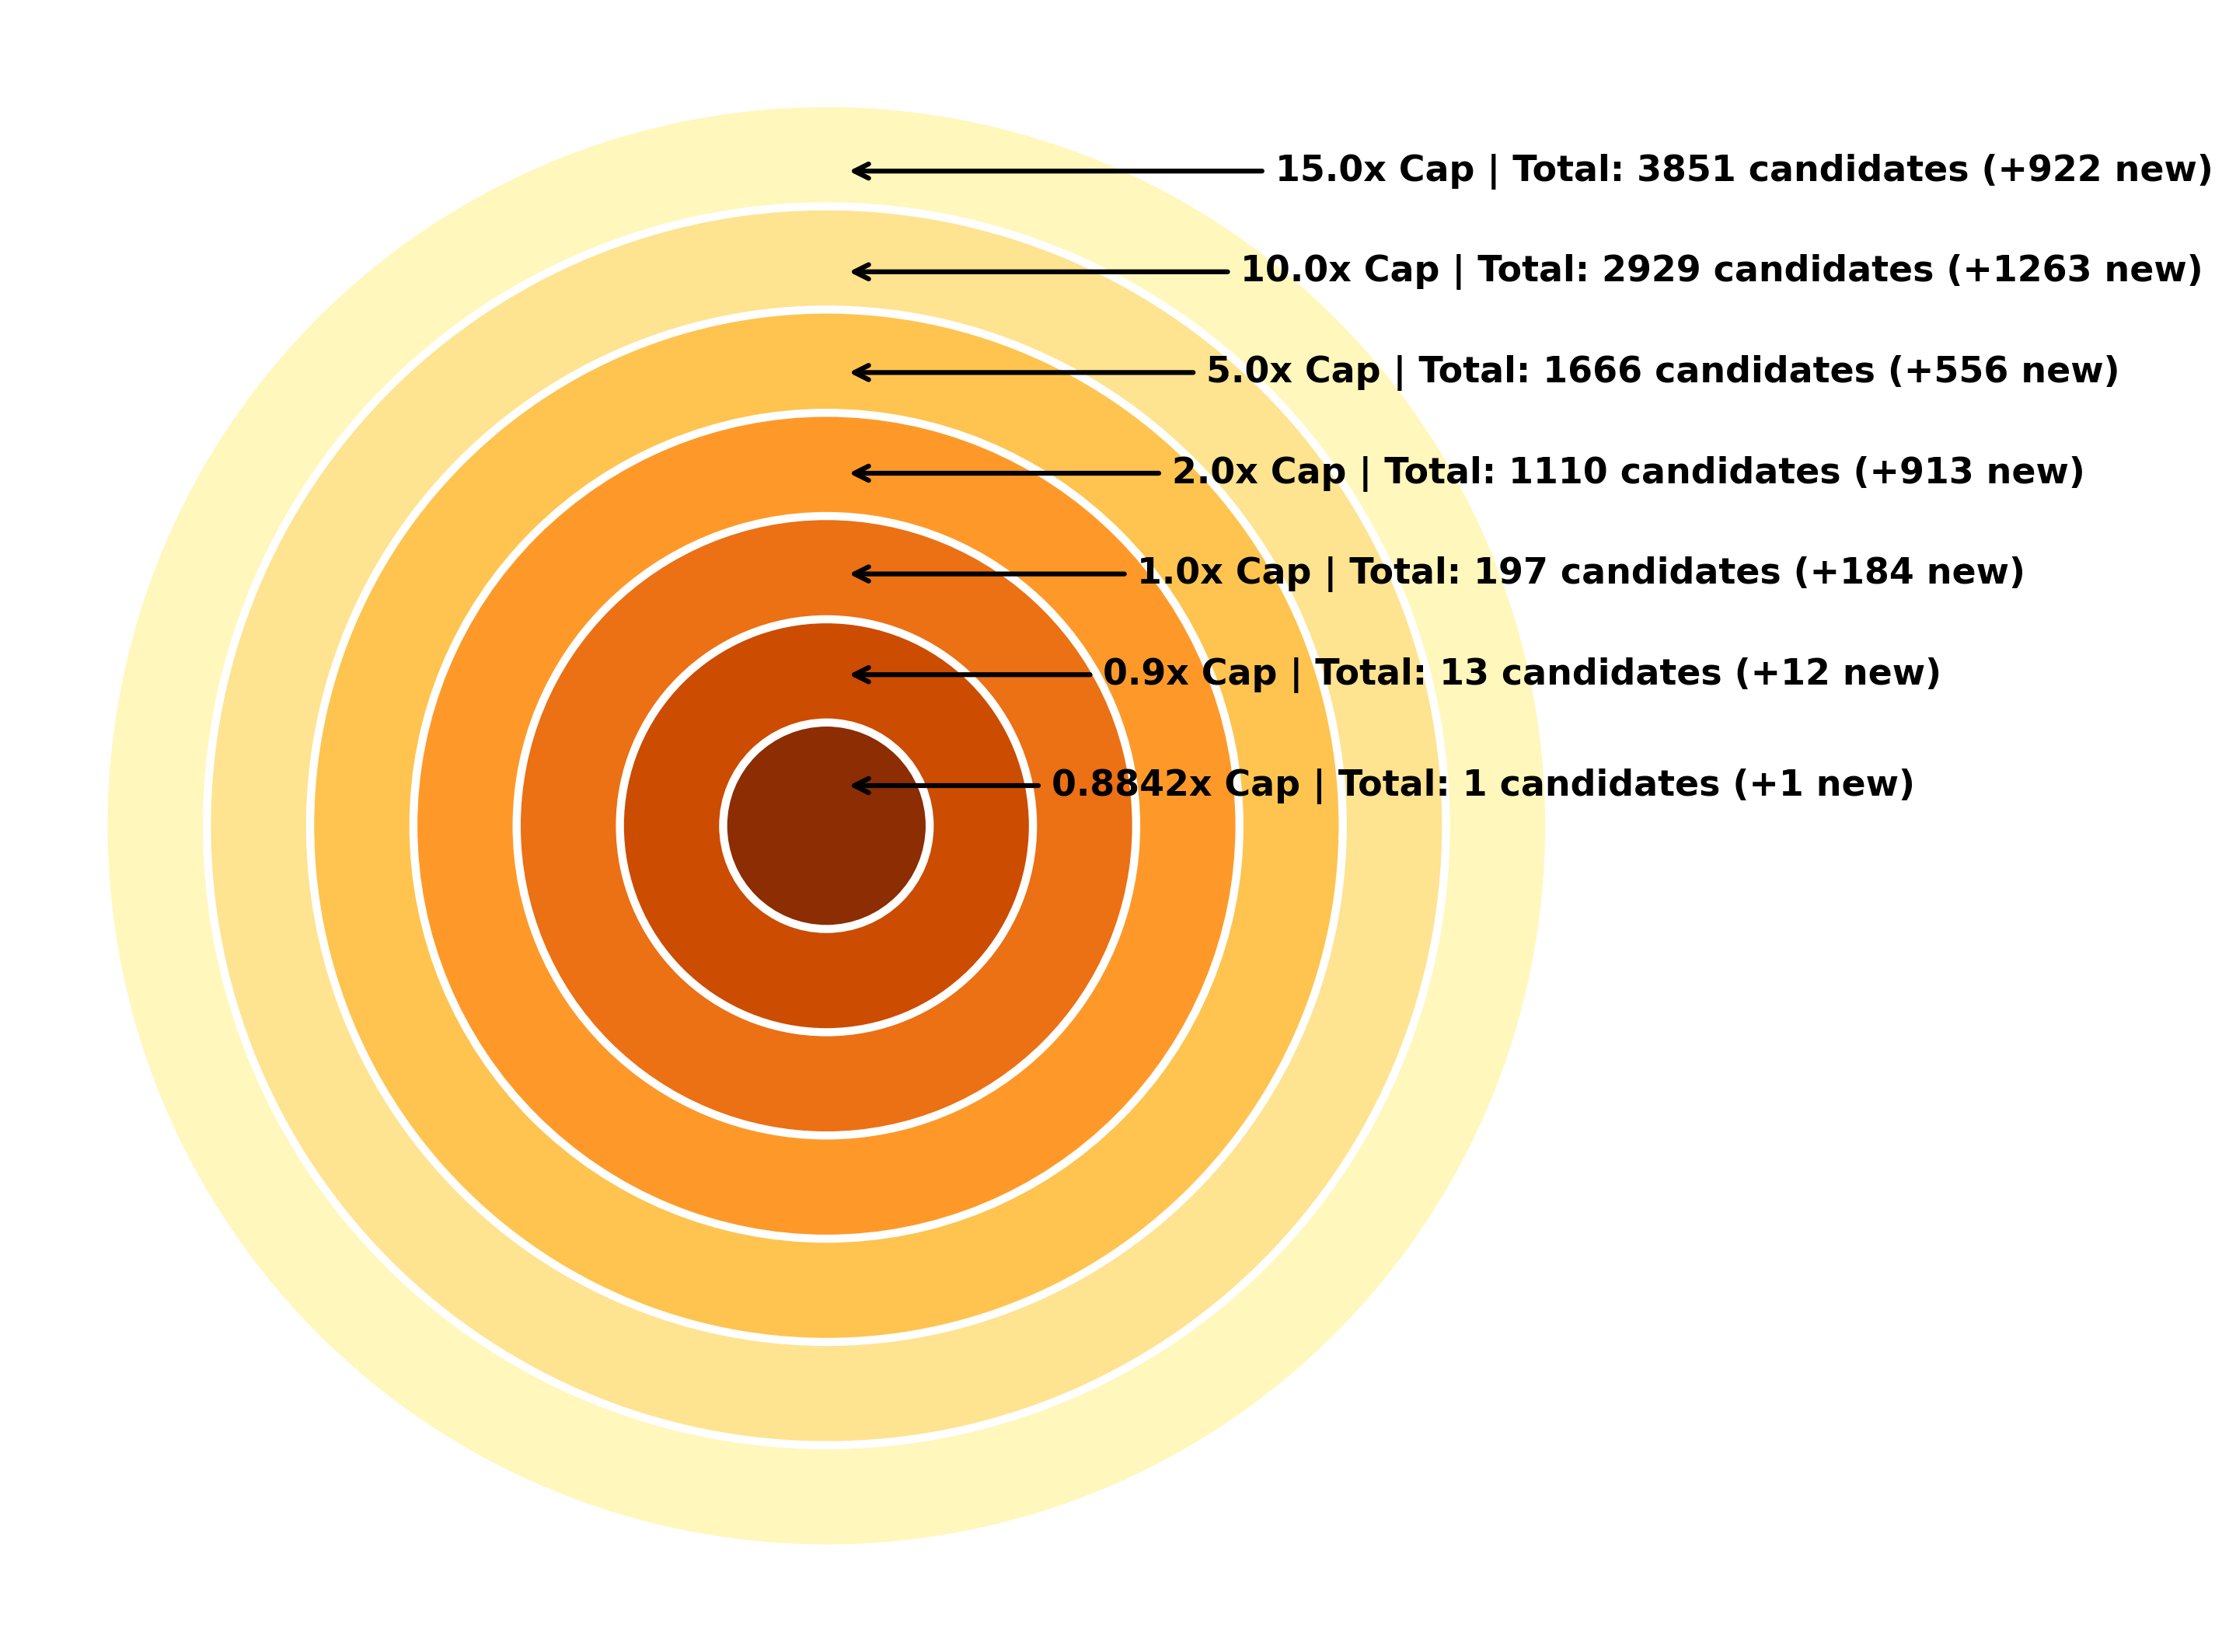
\includegraphics[width=0.8\textwidth]{content/images/concentric_diagram.png}
    \caption{Global Minimax Expansion: Concentric Euler diagram illustrating the volume of candidates unlocked at expanding uniform multiplier thresholds.}
    \label{fig:concentric_minimax}
\end{figure}

Naturally, the smaller the multiplier $X$, the fewer candidates survive the filter. A clear winner emerges at $X \approx 0.8842$; let us see how compelling it actually is (Table~\ref{tab:optimal_candidate_metrics}).

\begin{table}[h!]
    \centering
\small
\caption{Performance Comparison between the Standard Baseline and the Balanced Candidate}
\label{tab:optimal_candidate_metrics}
\begin{tabular}{lrrr}
\toprule
\textbf{Metric} & \textbf{Standard Baseline} & \textbf{Optimal Candidate} & \textbf{Ratio} \\
\midrule
        Parameters $(h, d, k, a, w)$ & $(63, 7, 14, 12, 16)$ & $(40, 5, 24, 8, 16)$ & -- \\
        Signature Size (Bytes) & $7{,}856$ & $6{,}912$ & $0.8798\times$ \\
        Key Generation Cost & $292{,}862$ & $146{,}430$ & $0.5000\times$ \\
        Signing Cost & $2{,}279{,}391$ & $756{,}689$ & $0.3320\times$ \\
        Verification Cost & $2{,}387$ & $1{,}857$ & $0.7780\times$ \\
        Compression per Byte ($\rho$) & $0.3038$ & $0.2686$ & $0.8842\times$ \\
\bottomrule
\end{tabular}
\end{table}

One might call this a reasonable result. We are less impressed: a 12\% saving on signature size is not particularly attractive on its own (the goal is to materially close the gap with Schnorr).

\subsubsection{Case 3: Adaptive Search}
The strategy is straightforward:
\begin{enumerate}
    \item Decide which sacrifices you are willing to make on each metric.
    \item Find the best candidate among those that remain.
\end{enumerate}

For step (1) we apply the filters introduced in Section~\ref{sec:sweep-strategy}. This subsection is dedicated to step (2).

Each candidate is uniquely defined by its tuple of metric values, so the search for an optimal candidate can be cast as finding the point closest to the origin in a five-dimensional space (analogous to a shortest-vector problem, but mercifully confined to a small set of survivors), where each axis represents one of our metrics. That is almost the whole story.

To build intuition, suppose we care about only two metrics - signature size and signature generation cost. We require the signature size to be no larger than that of SLH-DSA, and we are willing to tolerate a signing cost of at most $2\times$ the standard. In this case all admissible candidates fit inside the green rectangle in Figure~\ref{fig:scatter_plot}, which makes brute-force inspection easy: the best candidate is simply the point closest to the origin $(0, 0)$.

\begin{figure}[h!]
    \centering
    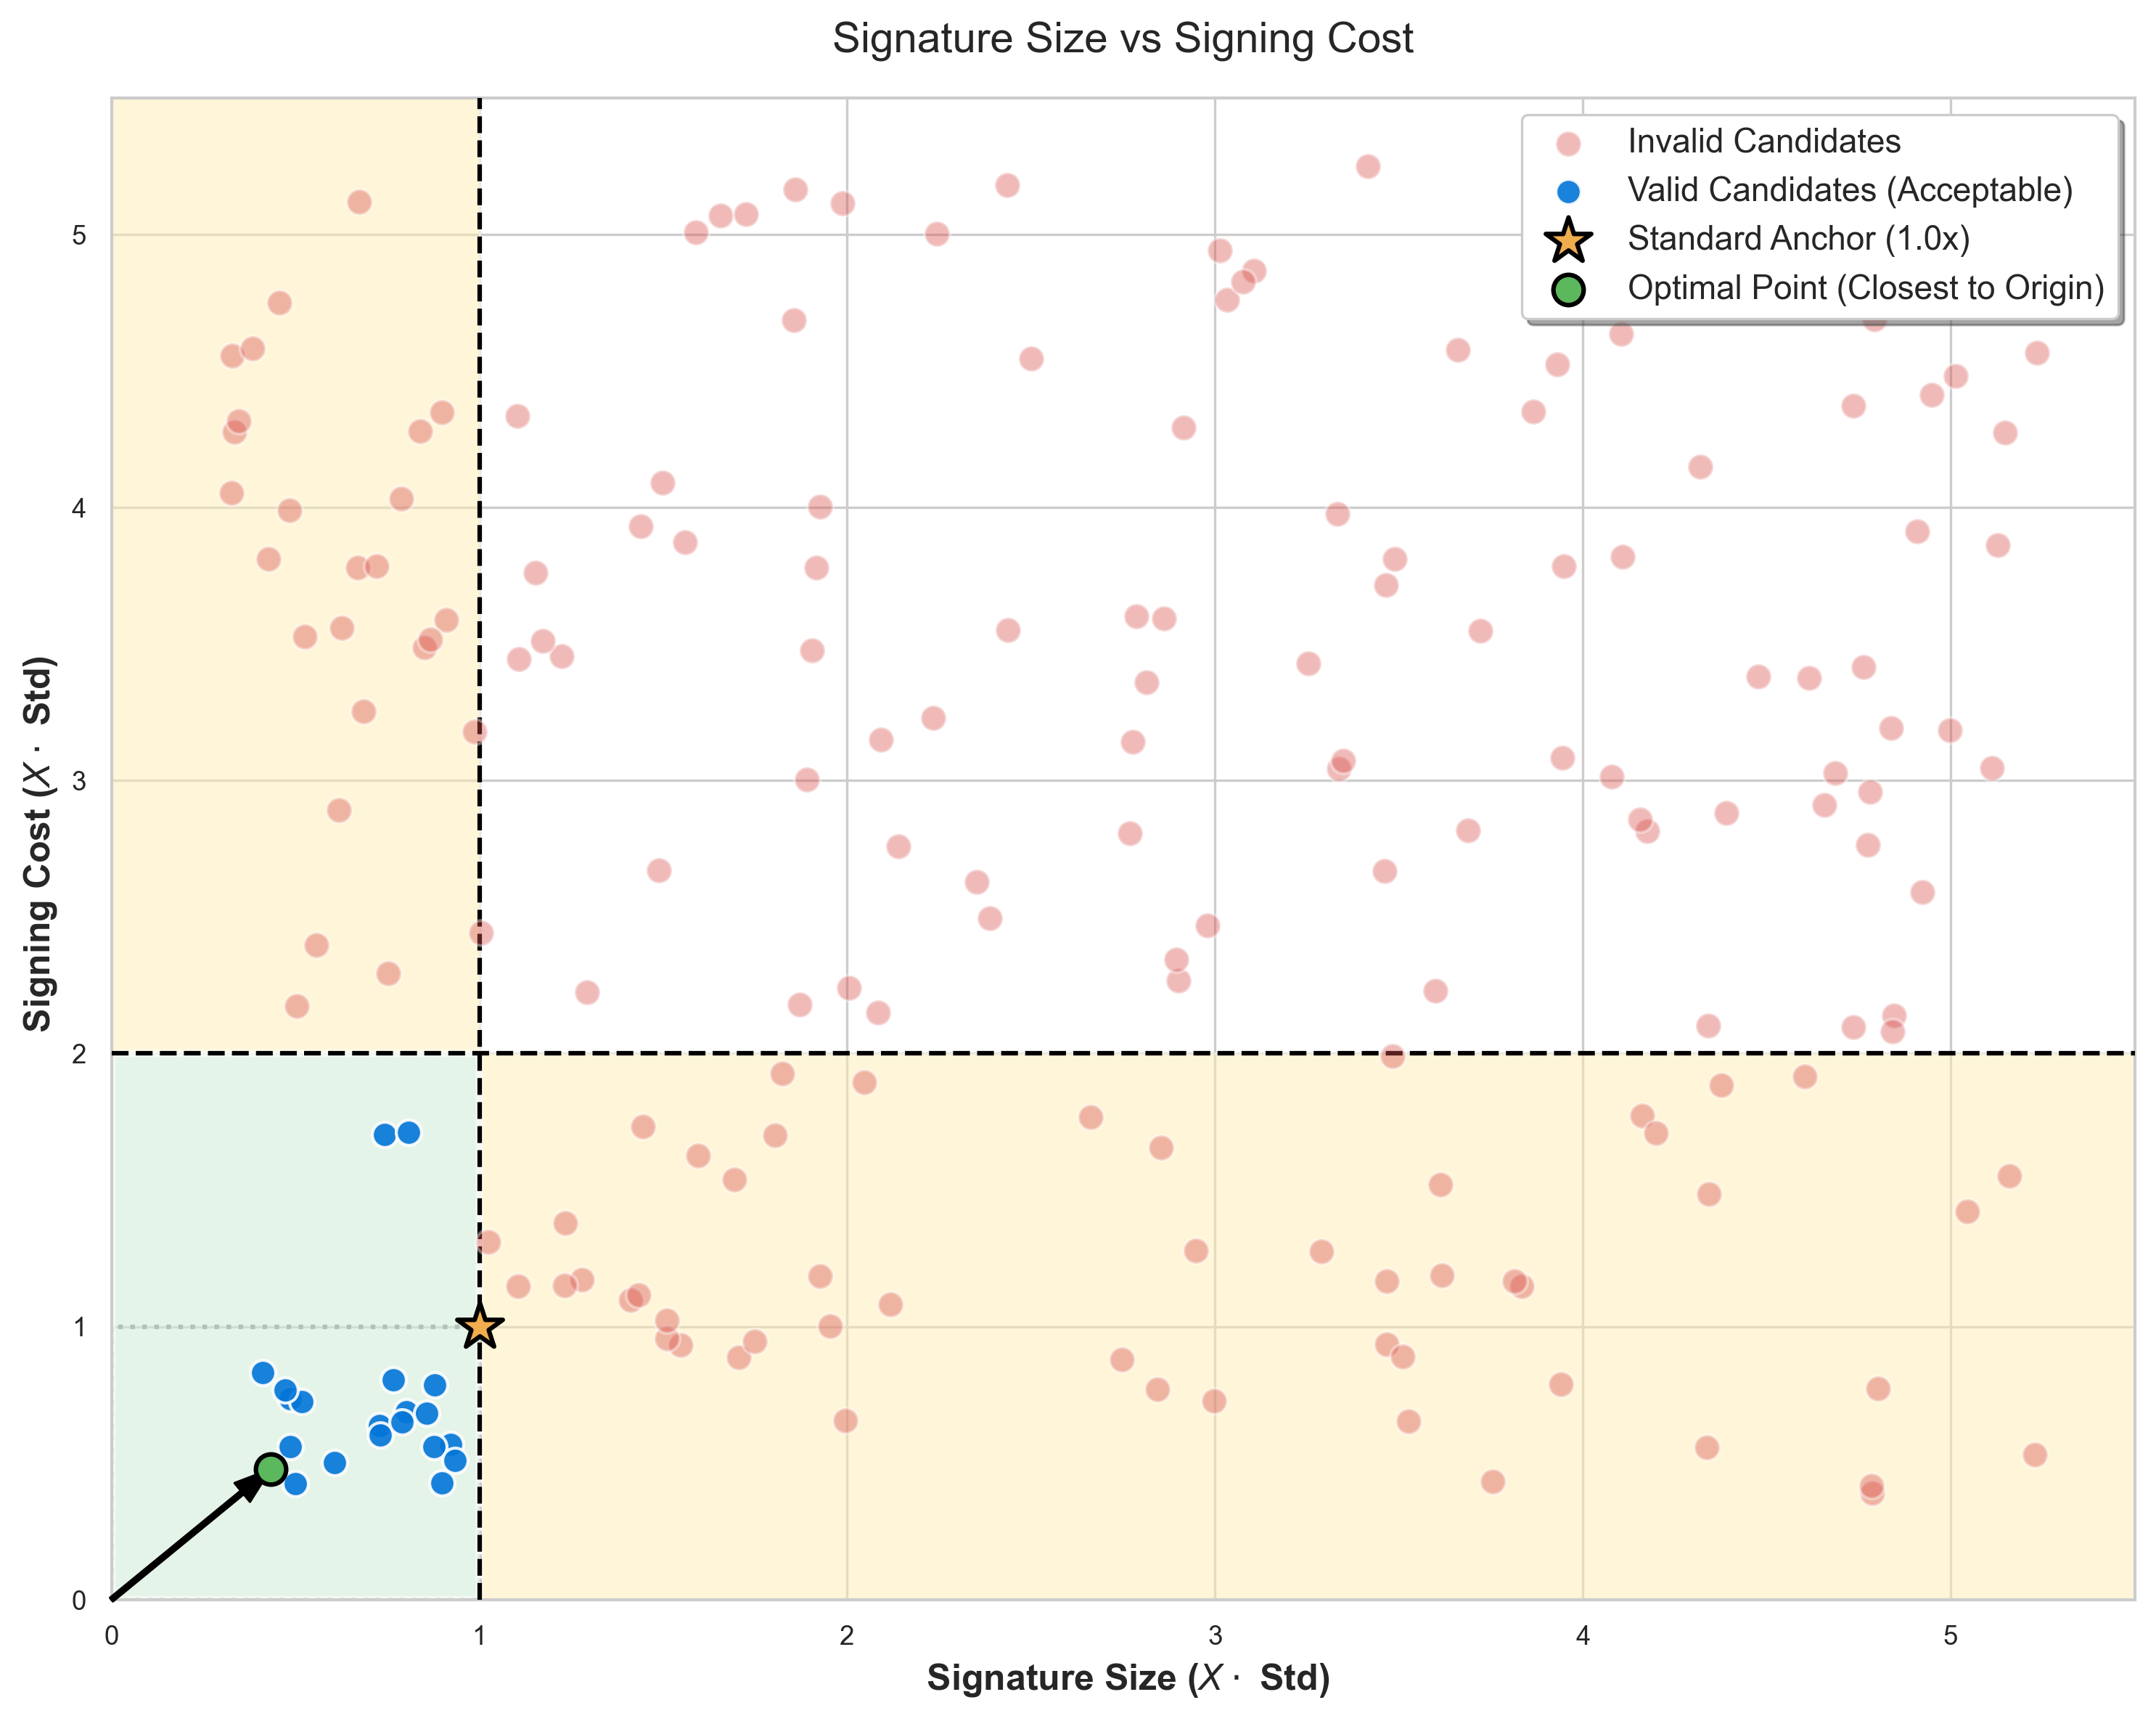
\includegraphics[width=0.7\textwidth]{content/images/scatter_plot.png}
    \caption{Visualization of Candidates with Prioritization of Size and Signing Cost Metrics.}
    \label{fig:scatter_plot}
\end{figure}

We cannot directly visualize a 5-dimensional space, but we can show the filtering process in a different way.

First, we scatter the unbounded candidate set (subject only to the 128-bit security condition) on a plane, with positions chosen randomly - the layout carries no meaning, and each point is uniquely identified by its parameter tuple. After initialization, we apply the signature-size filter, visualized as a coloured ``sieve''. We then apply each remaining filter in turn until the last one.

The resulting set contains the candidates that survived every filter; this is the pool in which we search for the best one.

As an example, consider the following filter coefficients:
\begin{equation*}
    X_{\text{size}} = 0.85, \quad X_{\text{kg}} = 1.5, \quad X_{\text{sg}} = 2, \quad X_{\text{sv}} = 0.8, \quad X_{\text{cb}} = 1.
\end{equation*}

The filtering process is shown in Figure~\ref{fig:full_filtering_process}.

\begin{figure}[h!]
    \centering
    % Row 1
    \begin{subfigure}[b]{0.32\textwidth}
        \centering
        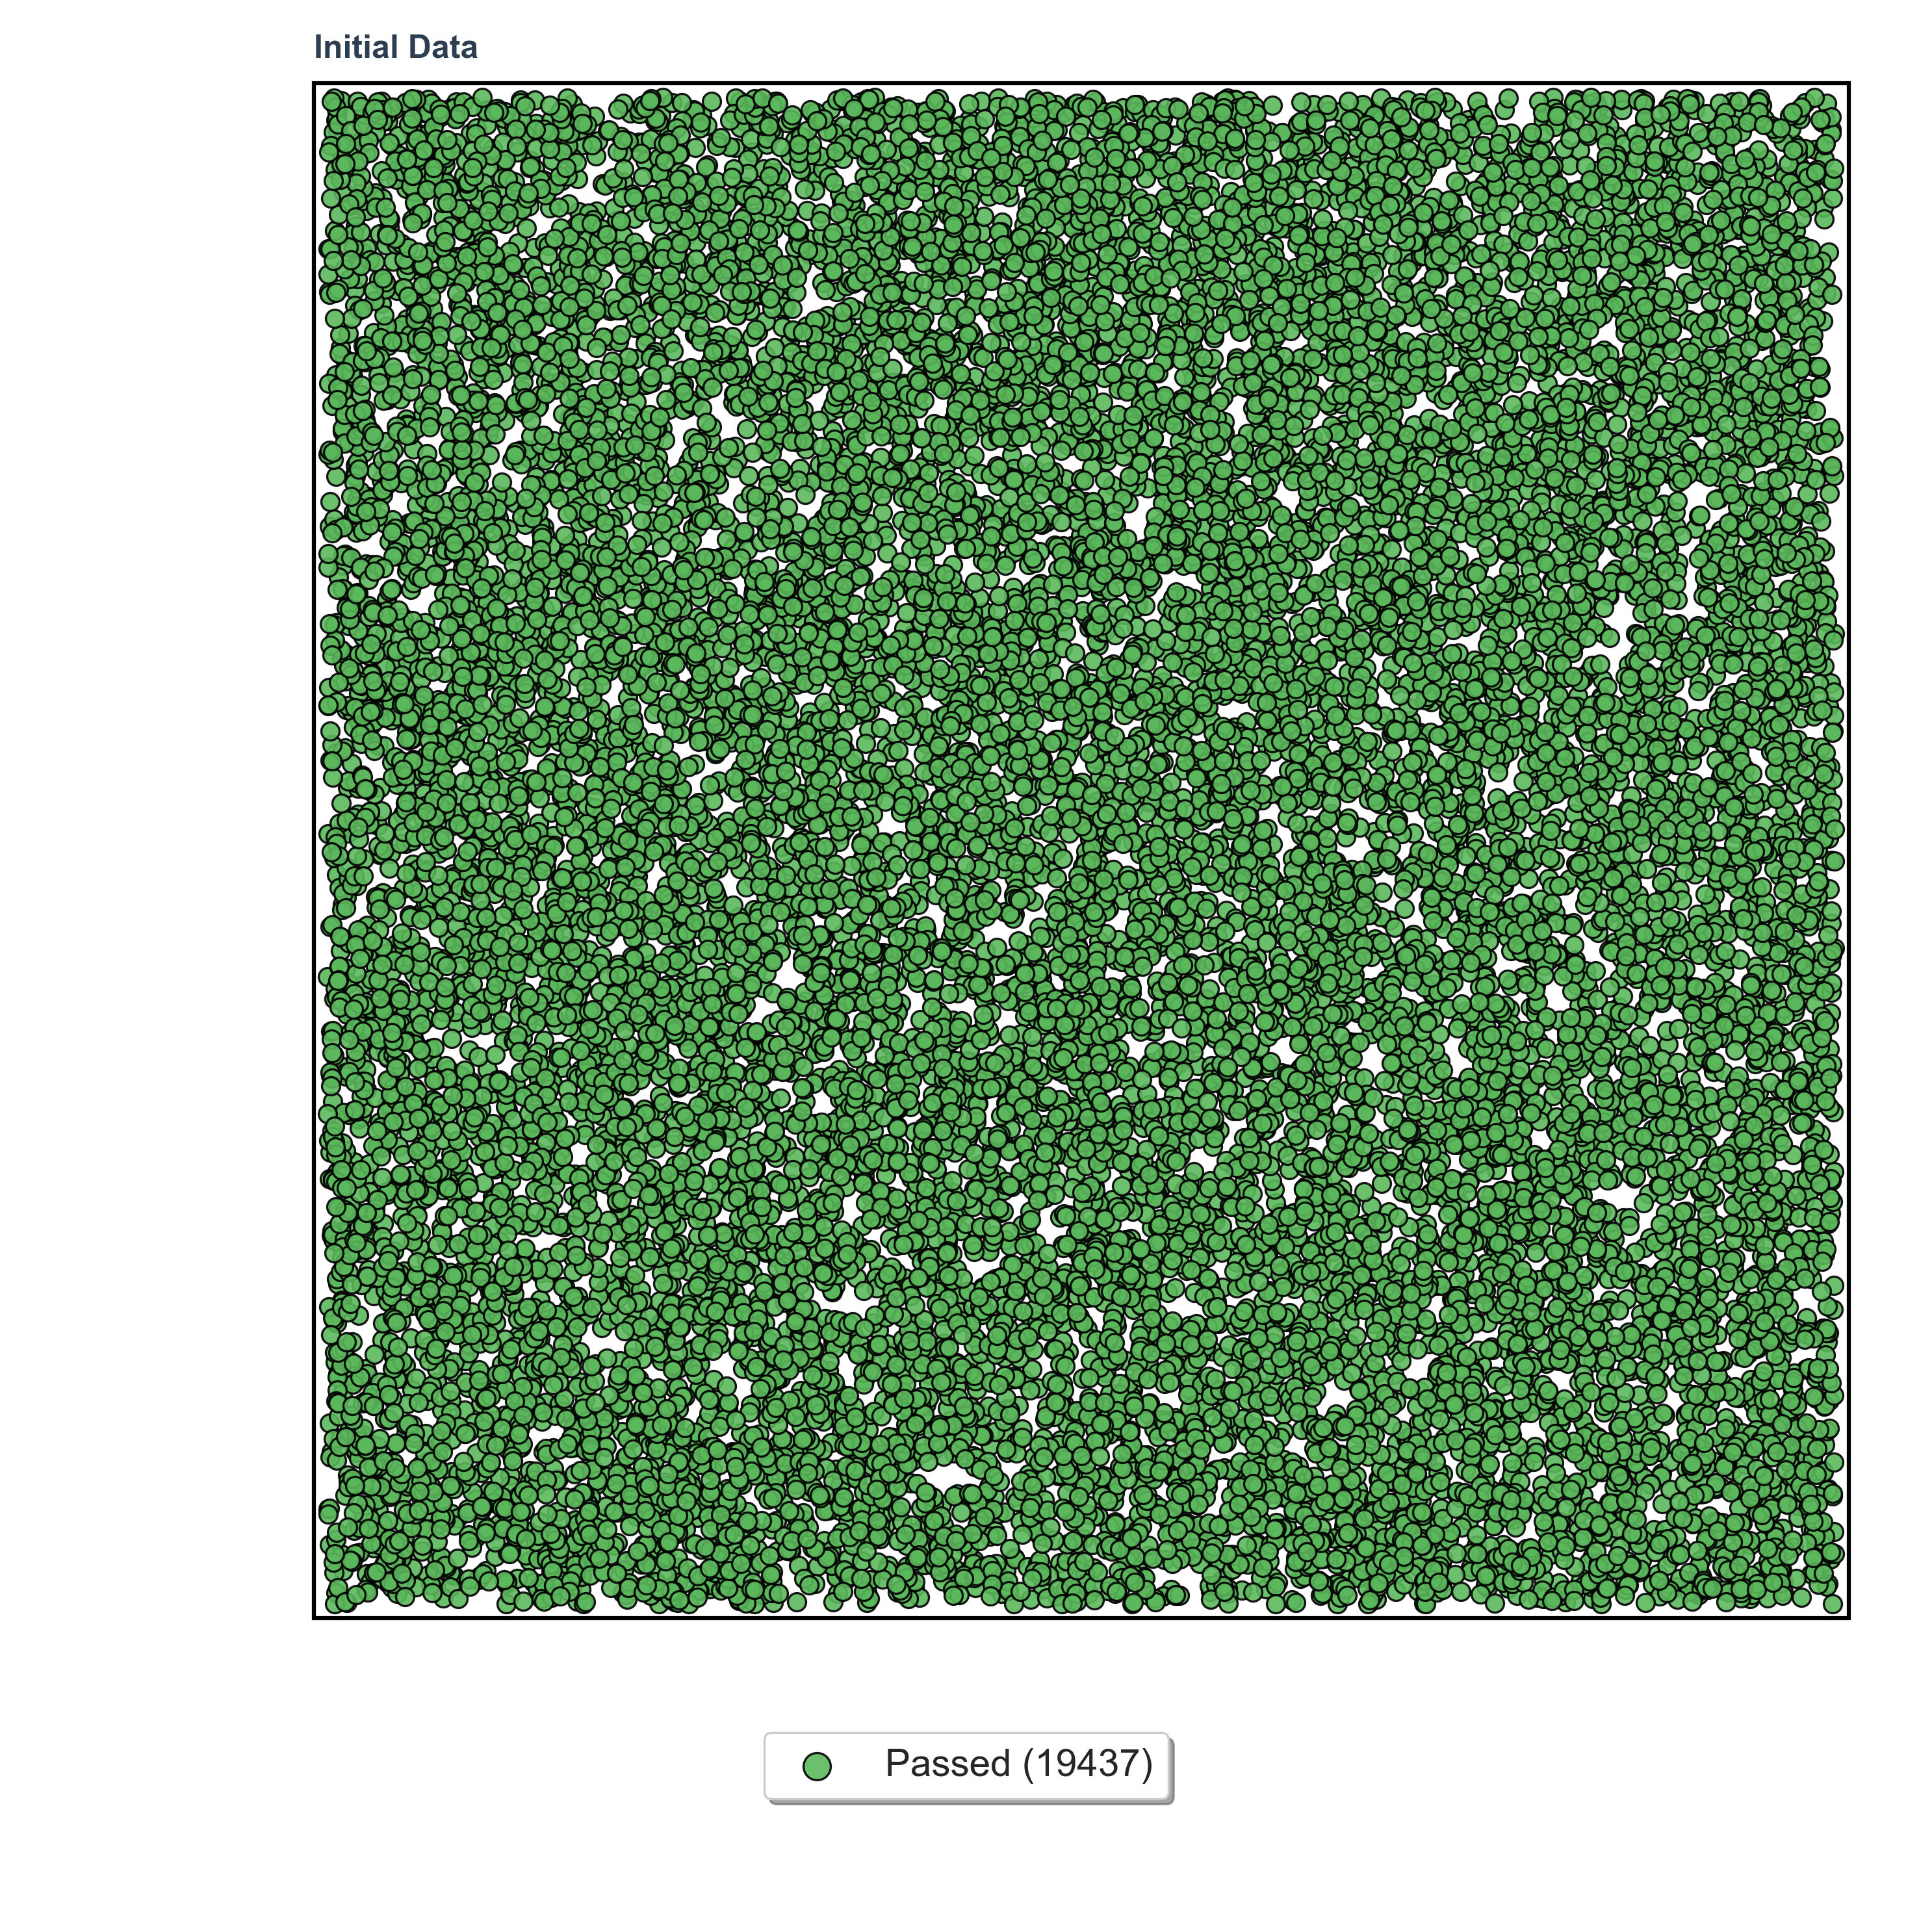
\includegraphics[width=\textwidth]{content/images/sieve_step1_initial.png}
        \caption{Initial Pool}
        \label{fig:sieve_1}
    \end{subfigure}
    \hfill
    \begin{subfigure}[b]{0.32\textwidth}
        \centering
        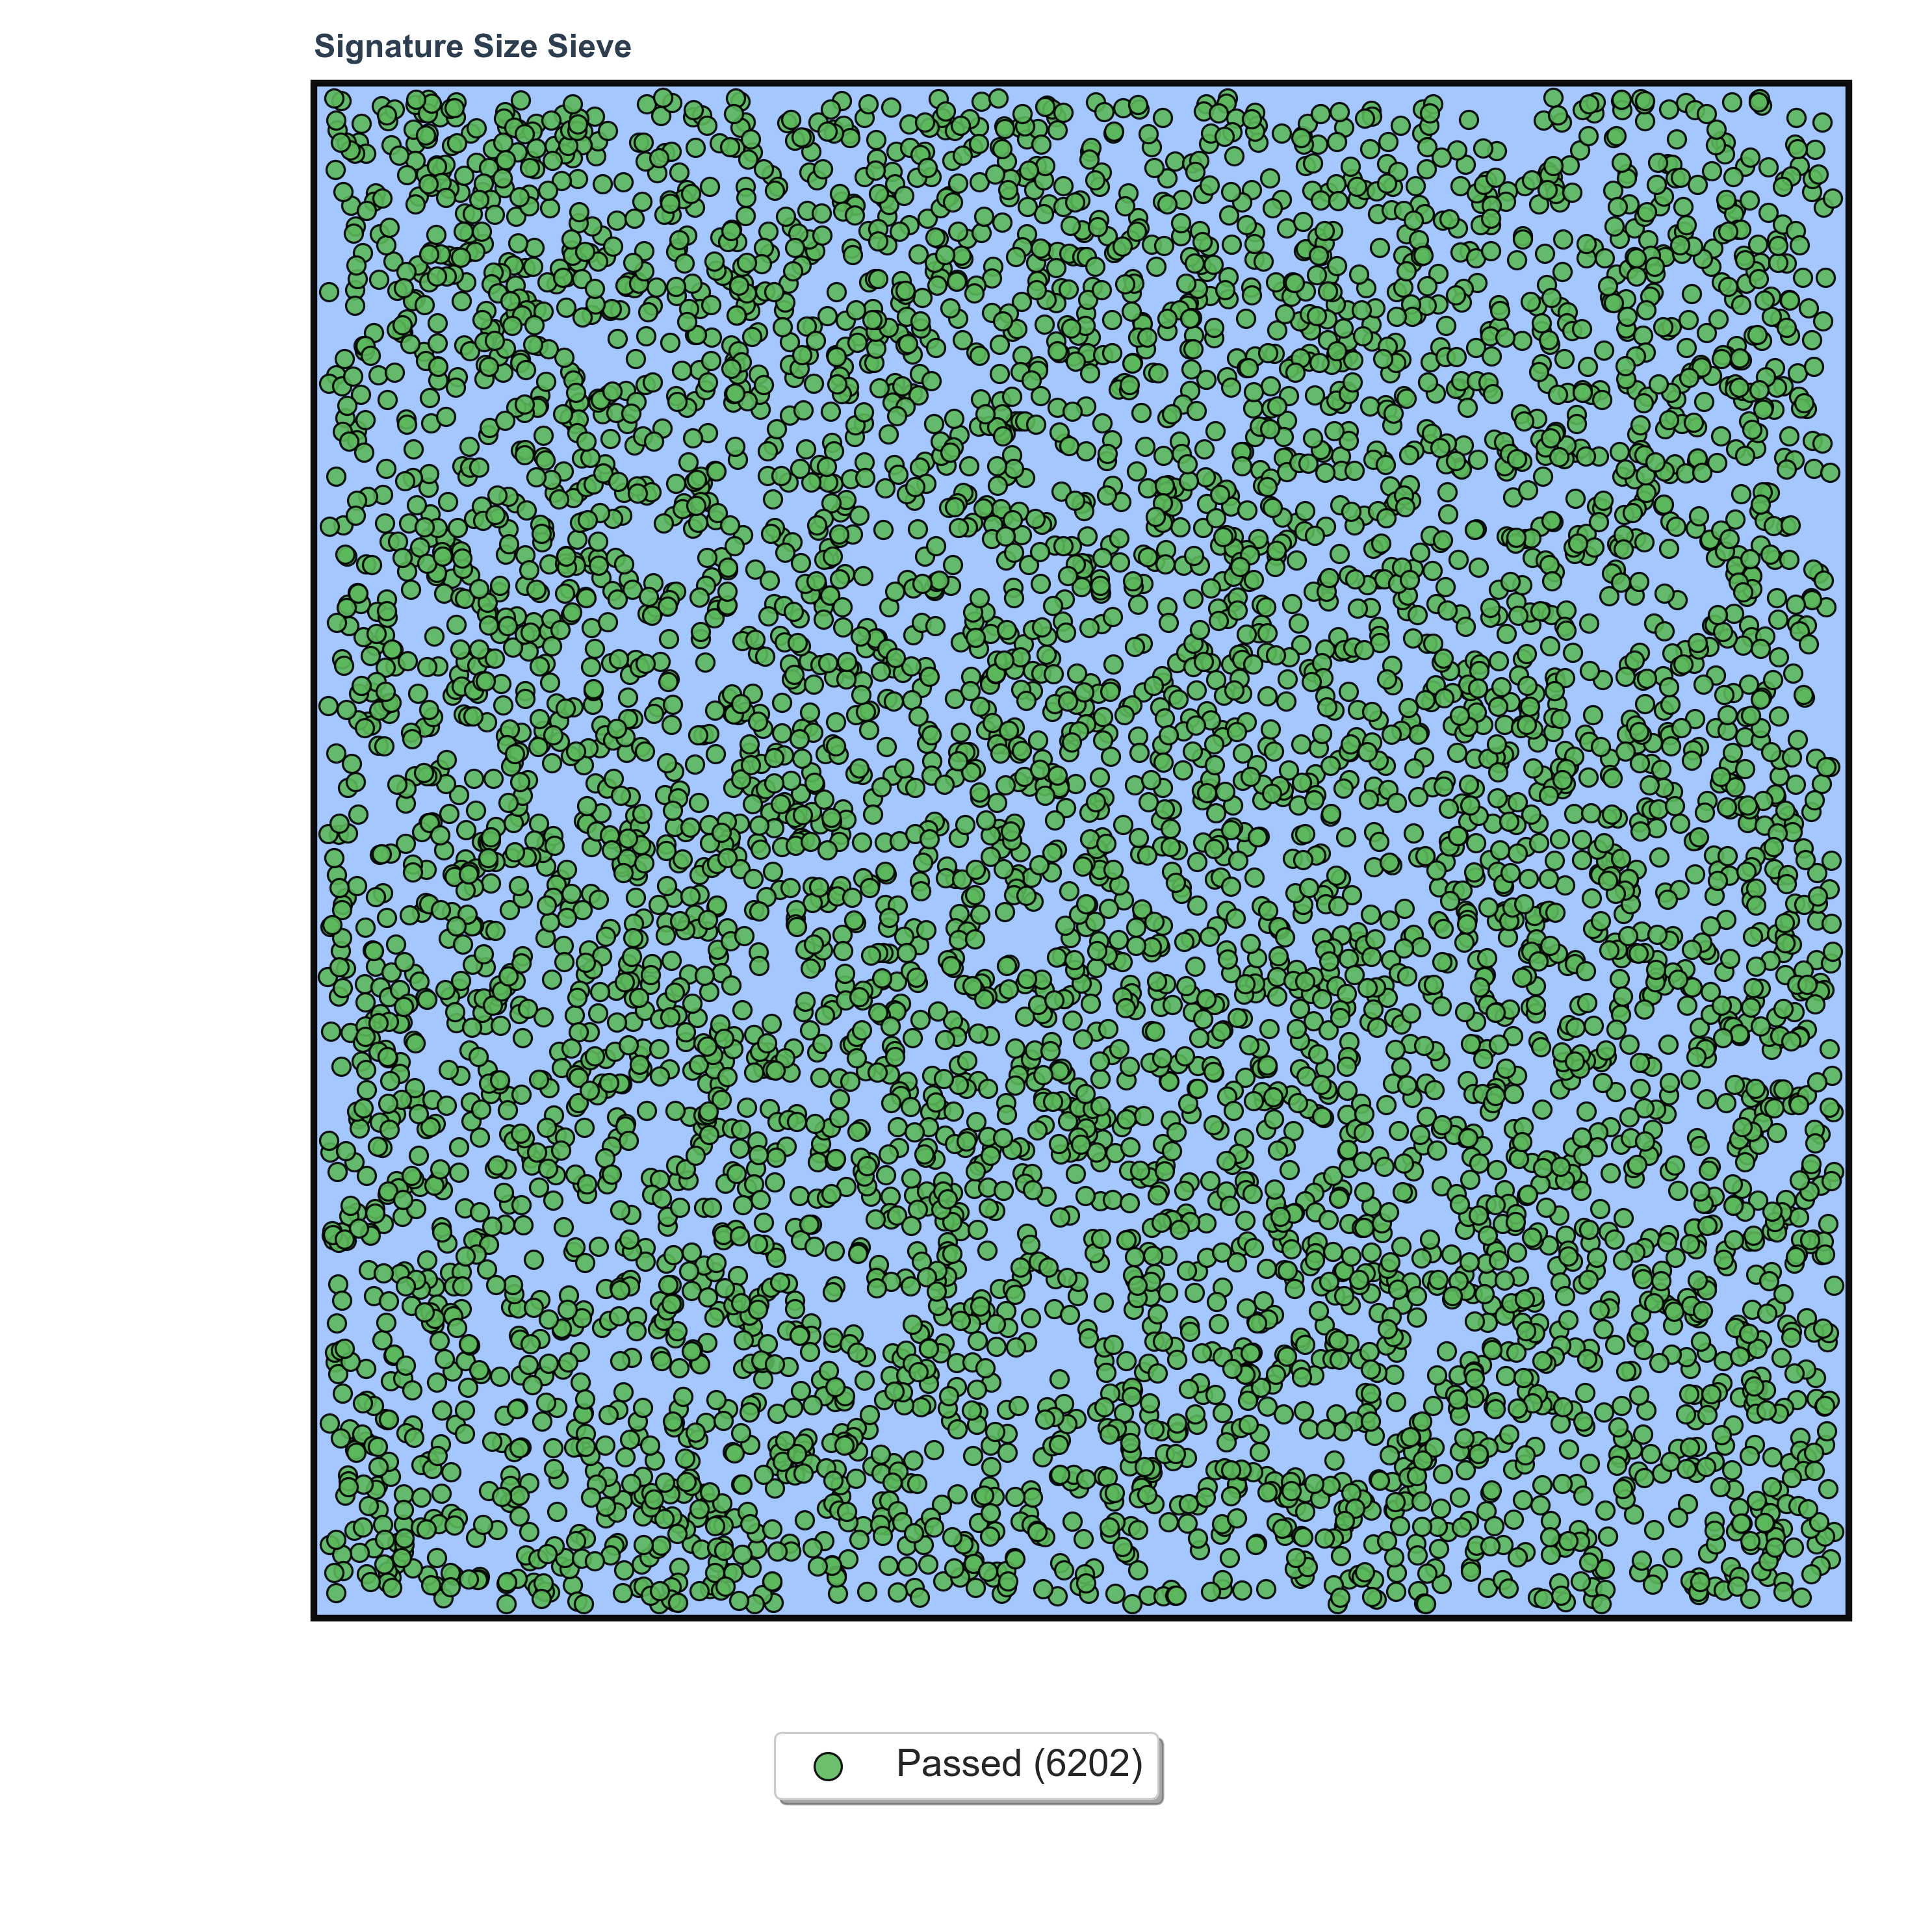
\includegraphics[width=\textwidth]{content/images/sieve_step2_size.png}
        \caption{SigSize}
        \label{fig:sieve_2}
    \end{subfigure}
    \hfill
    \begin{subfigure}[b]{0.32\textwidth}
        \centering
        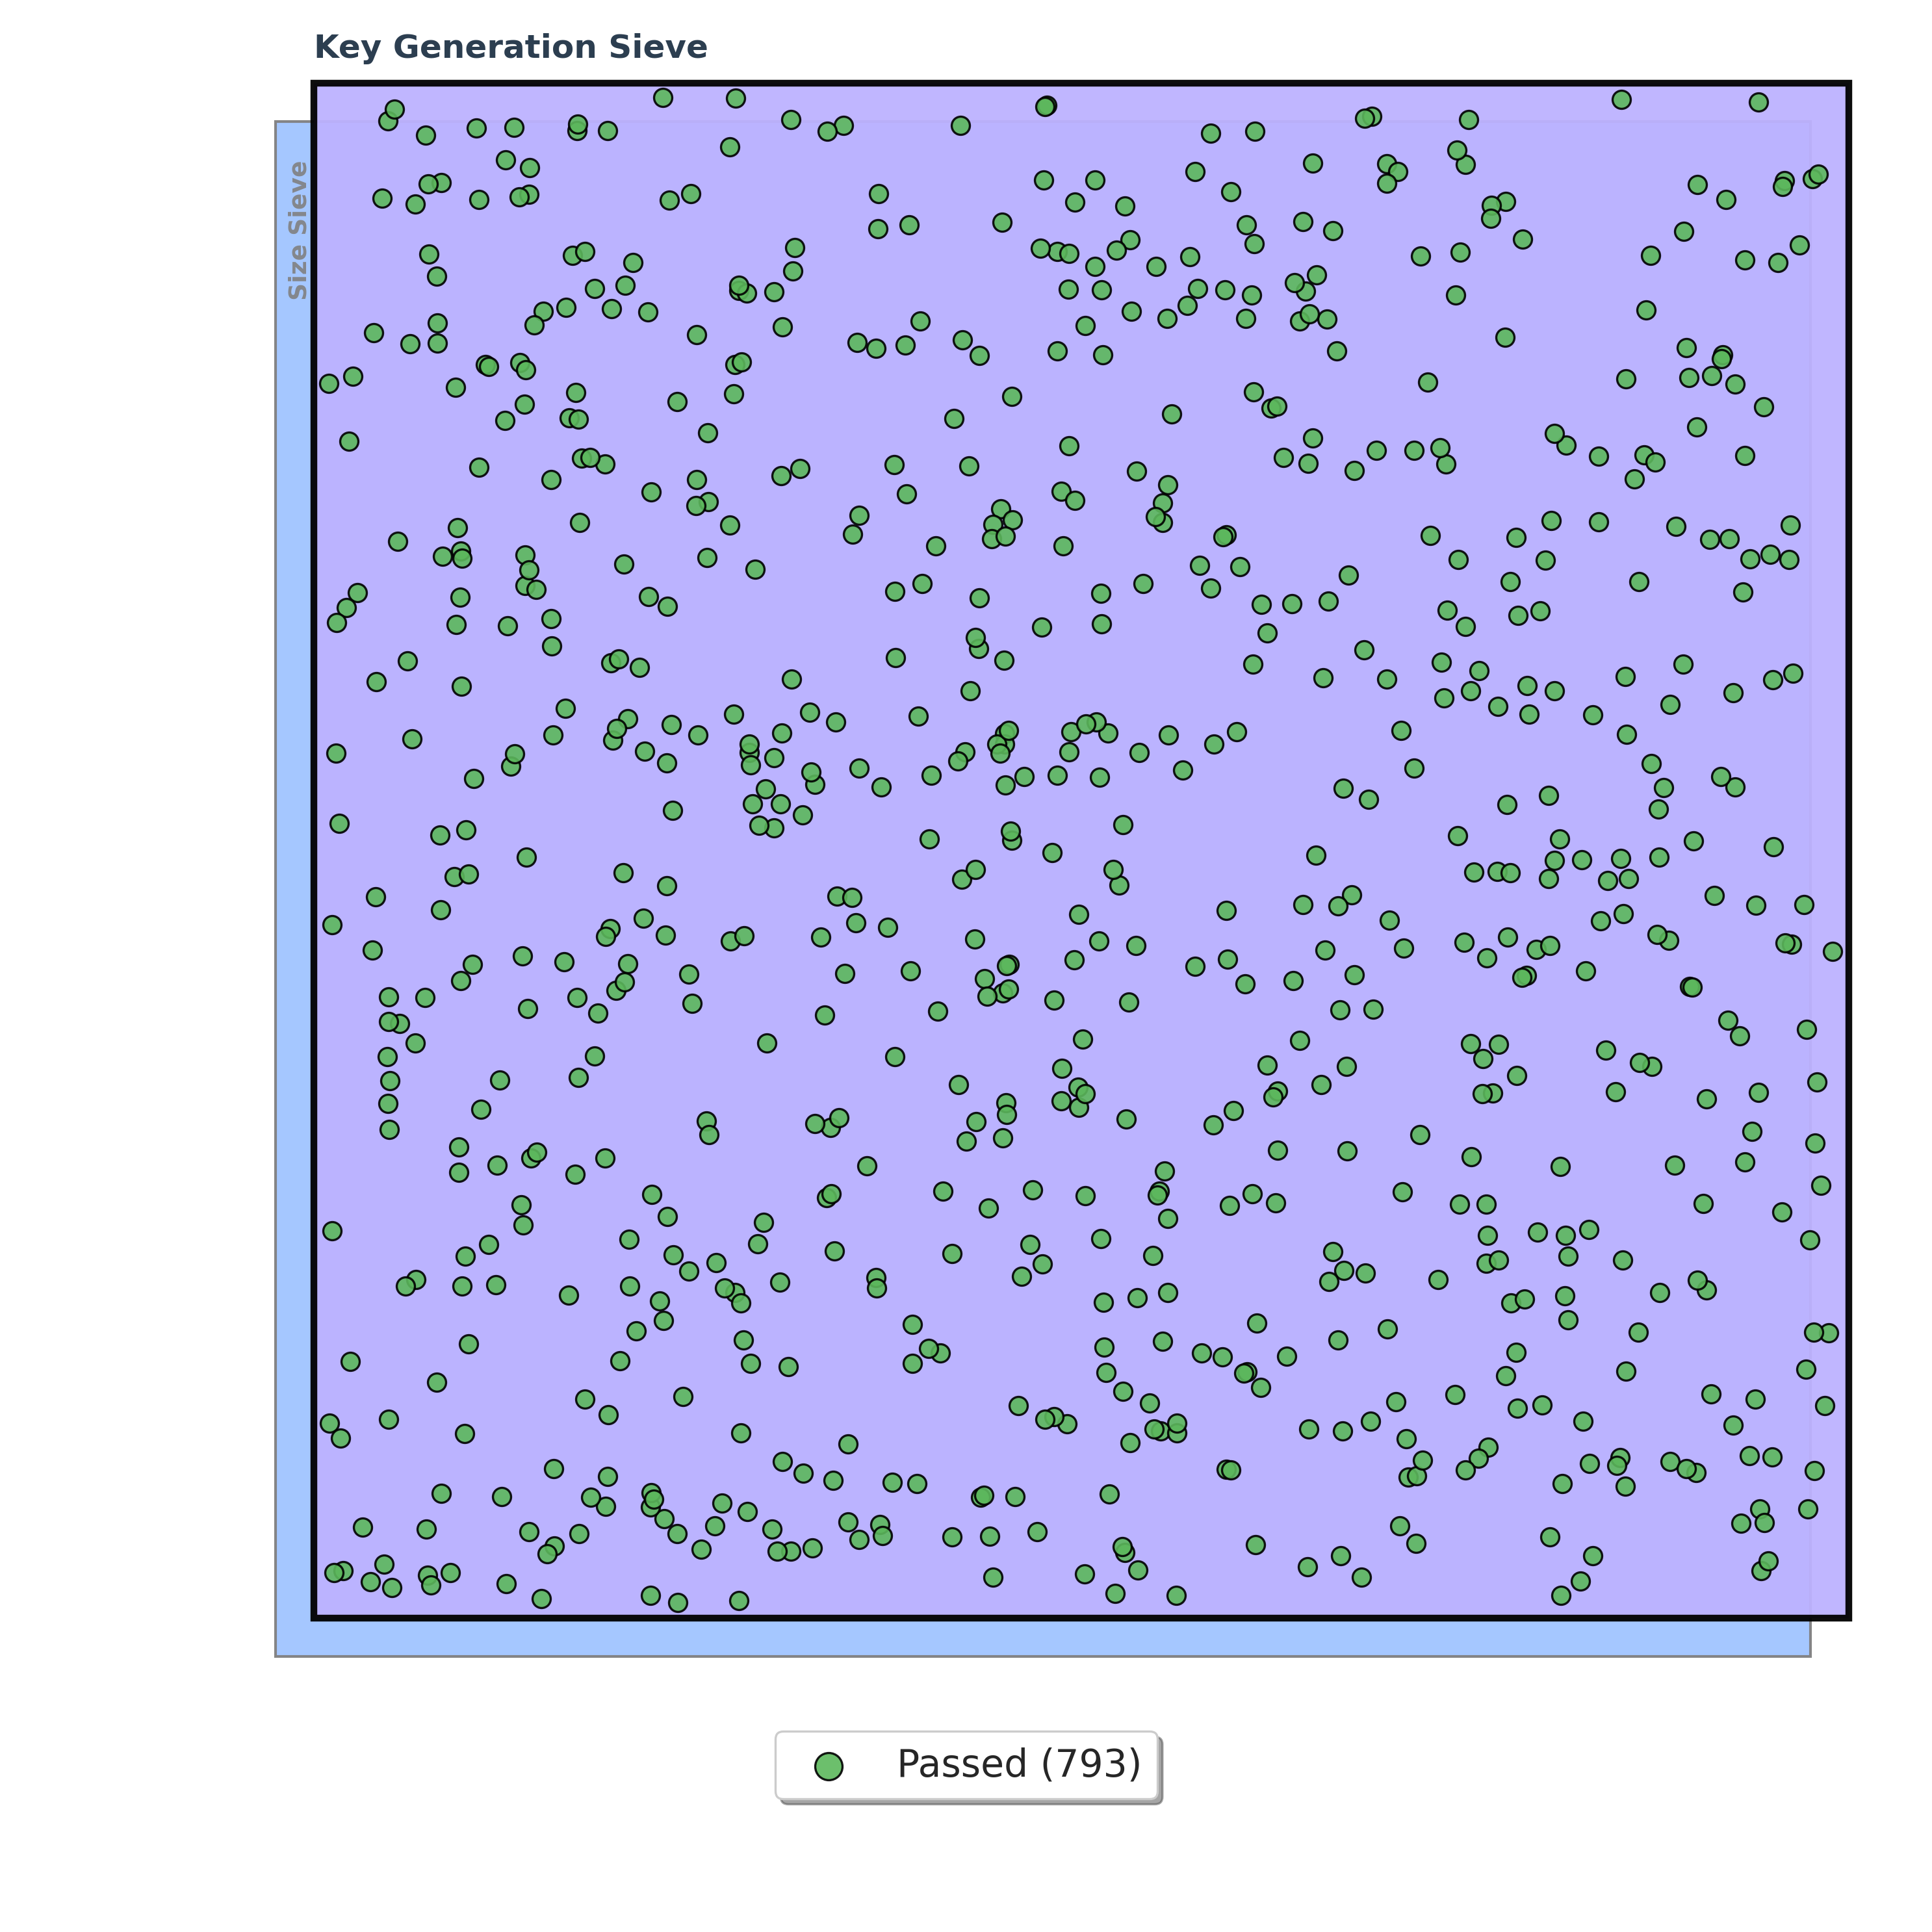
\includegraphics[width=\textwidth]{content/images/sieve_step3_keygen.png}
        \caption{KeyGen}
        \label{fig:sieve_3}
    \end{subfigure}
    
    \vspace{0.5cm}
    
    % Row 2
    \begin{subfigure}[b]{0.32\textwidth}
        \centering
        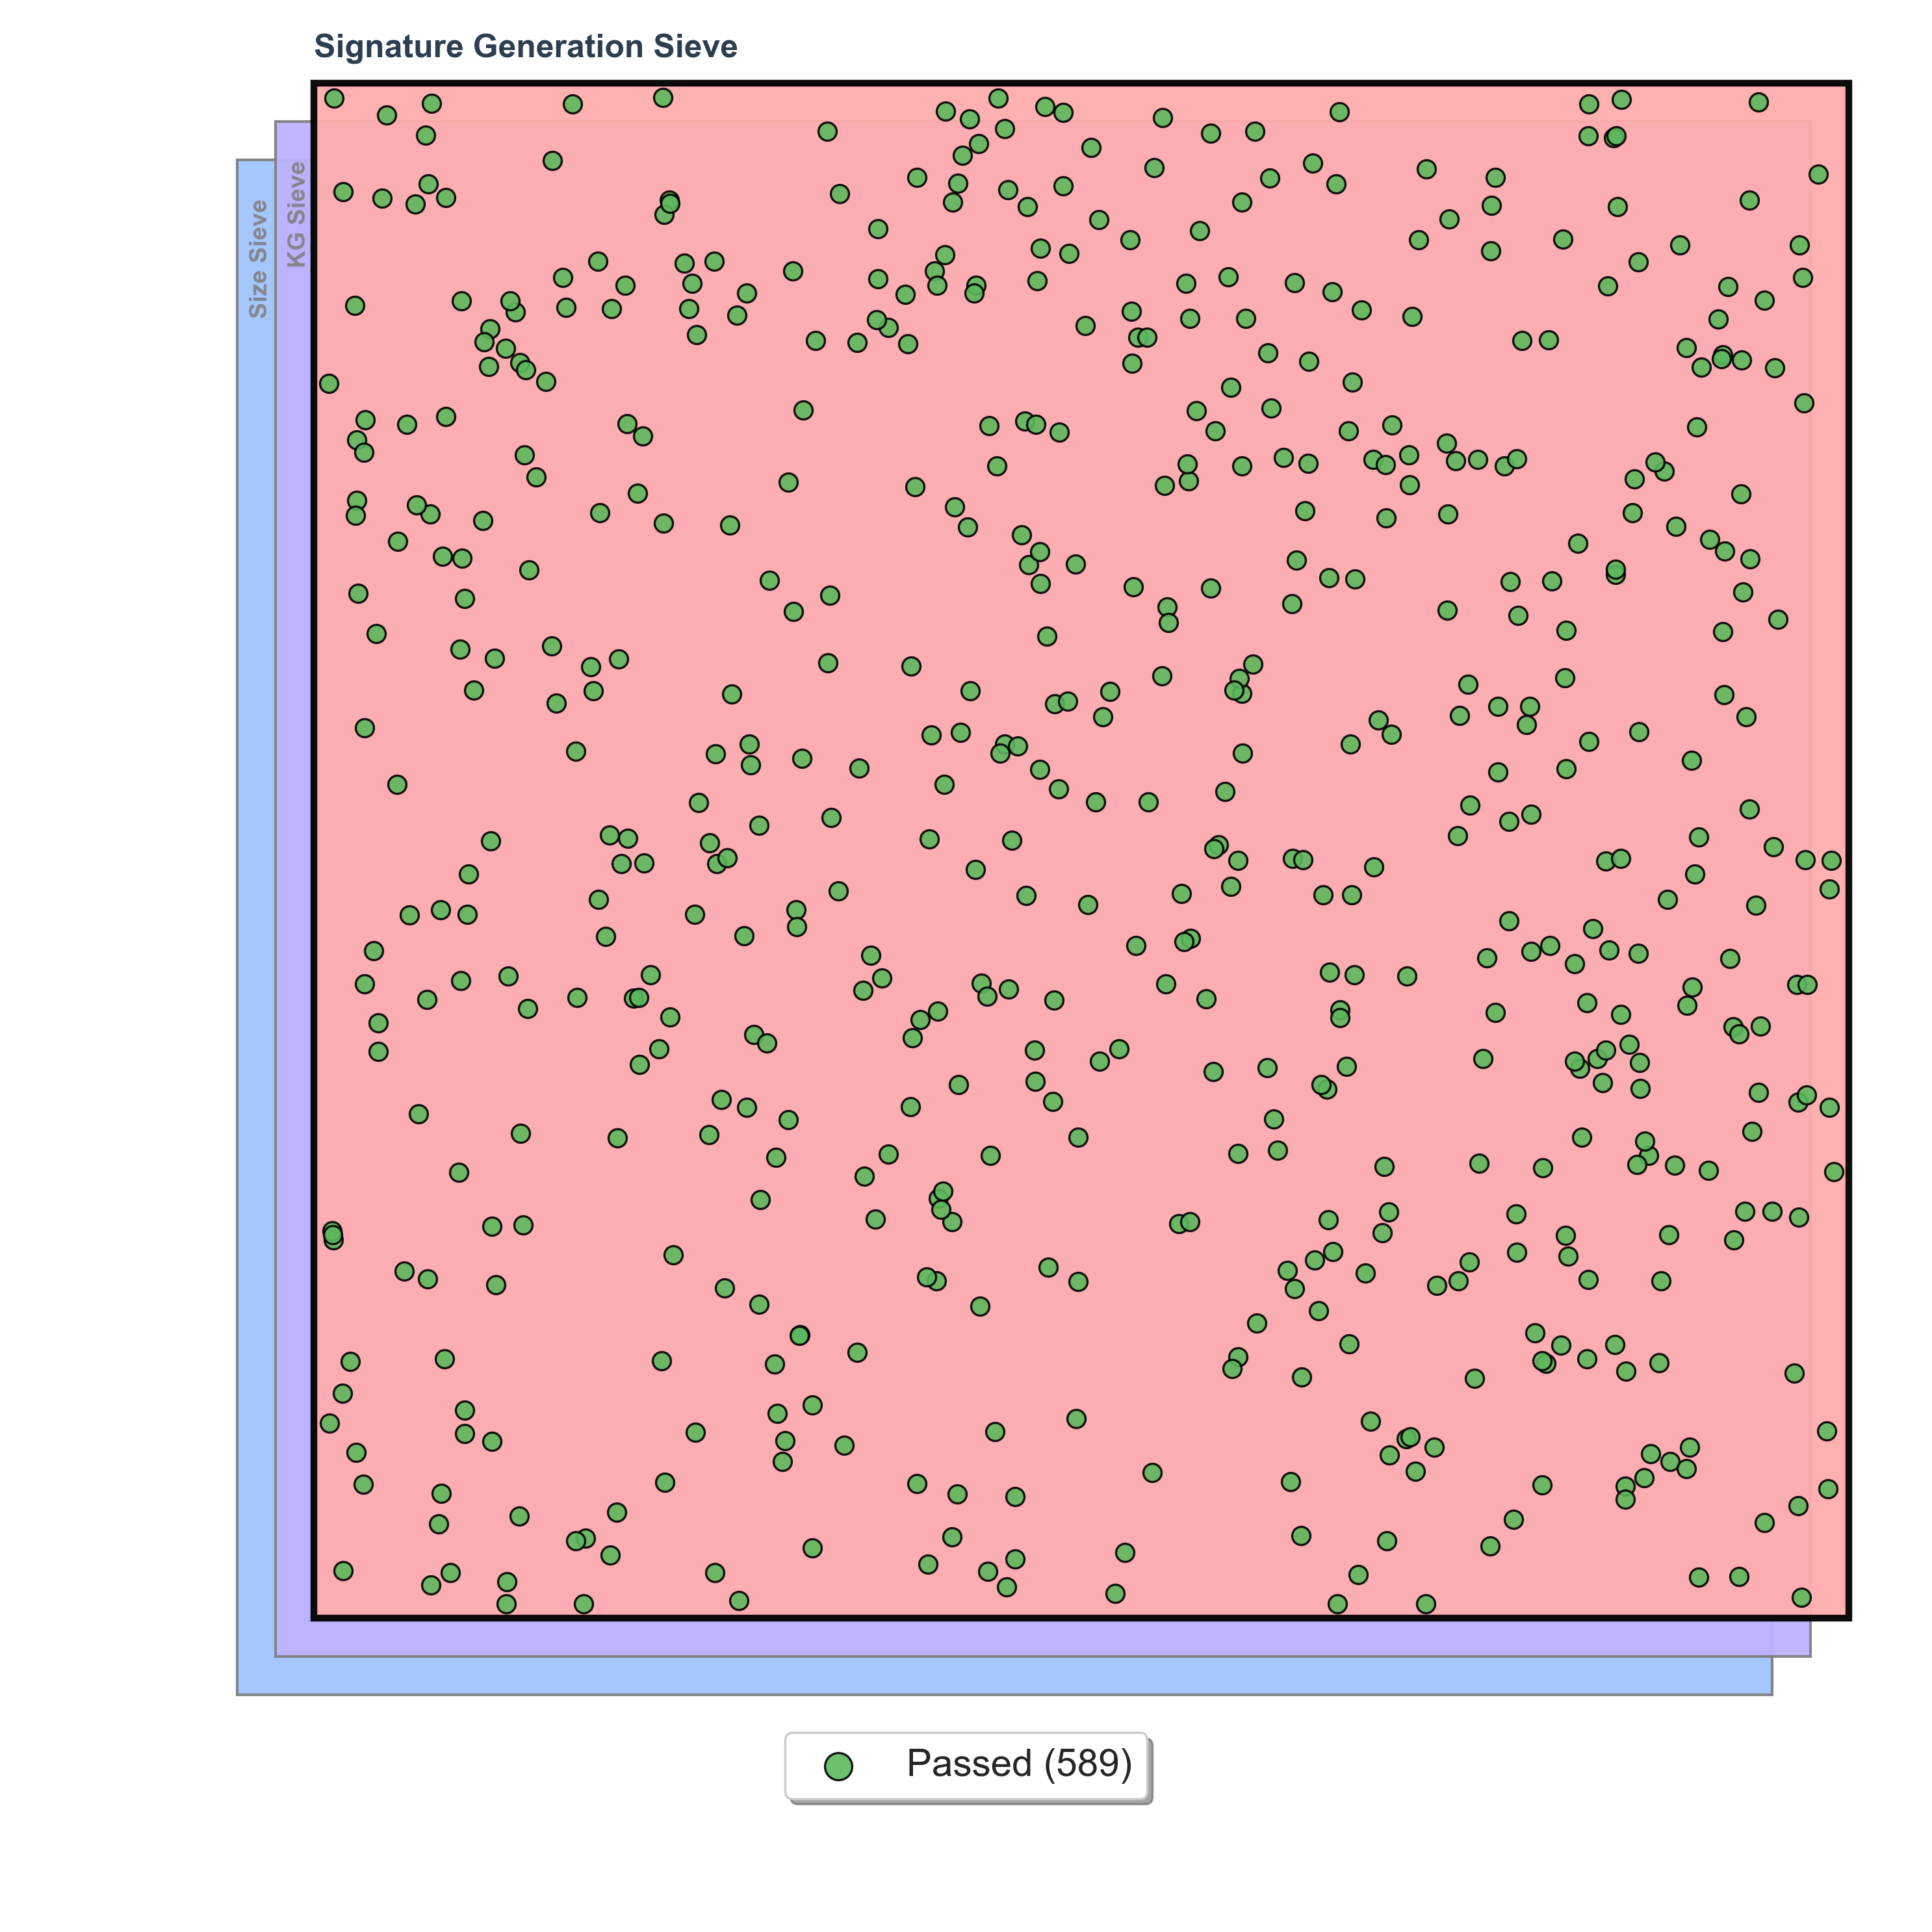
\includegraphics[width=\textwidth]{content/images/sieve_step4_siggen.png}
        \caption{SigGen}
        \label{fig:sieve_4}
    \end{subfigure}
    \hfill
    \begin{subfigure}[b]{0.32\textwidth}
        \centering
        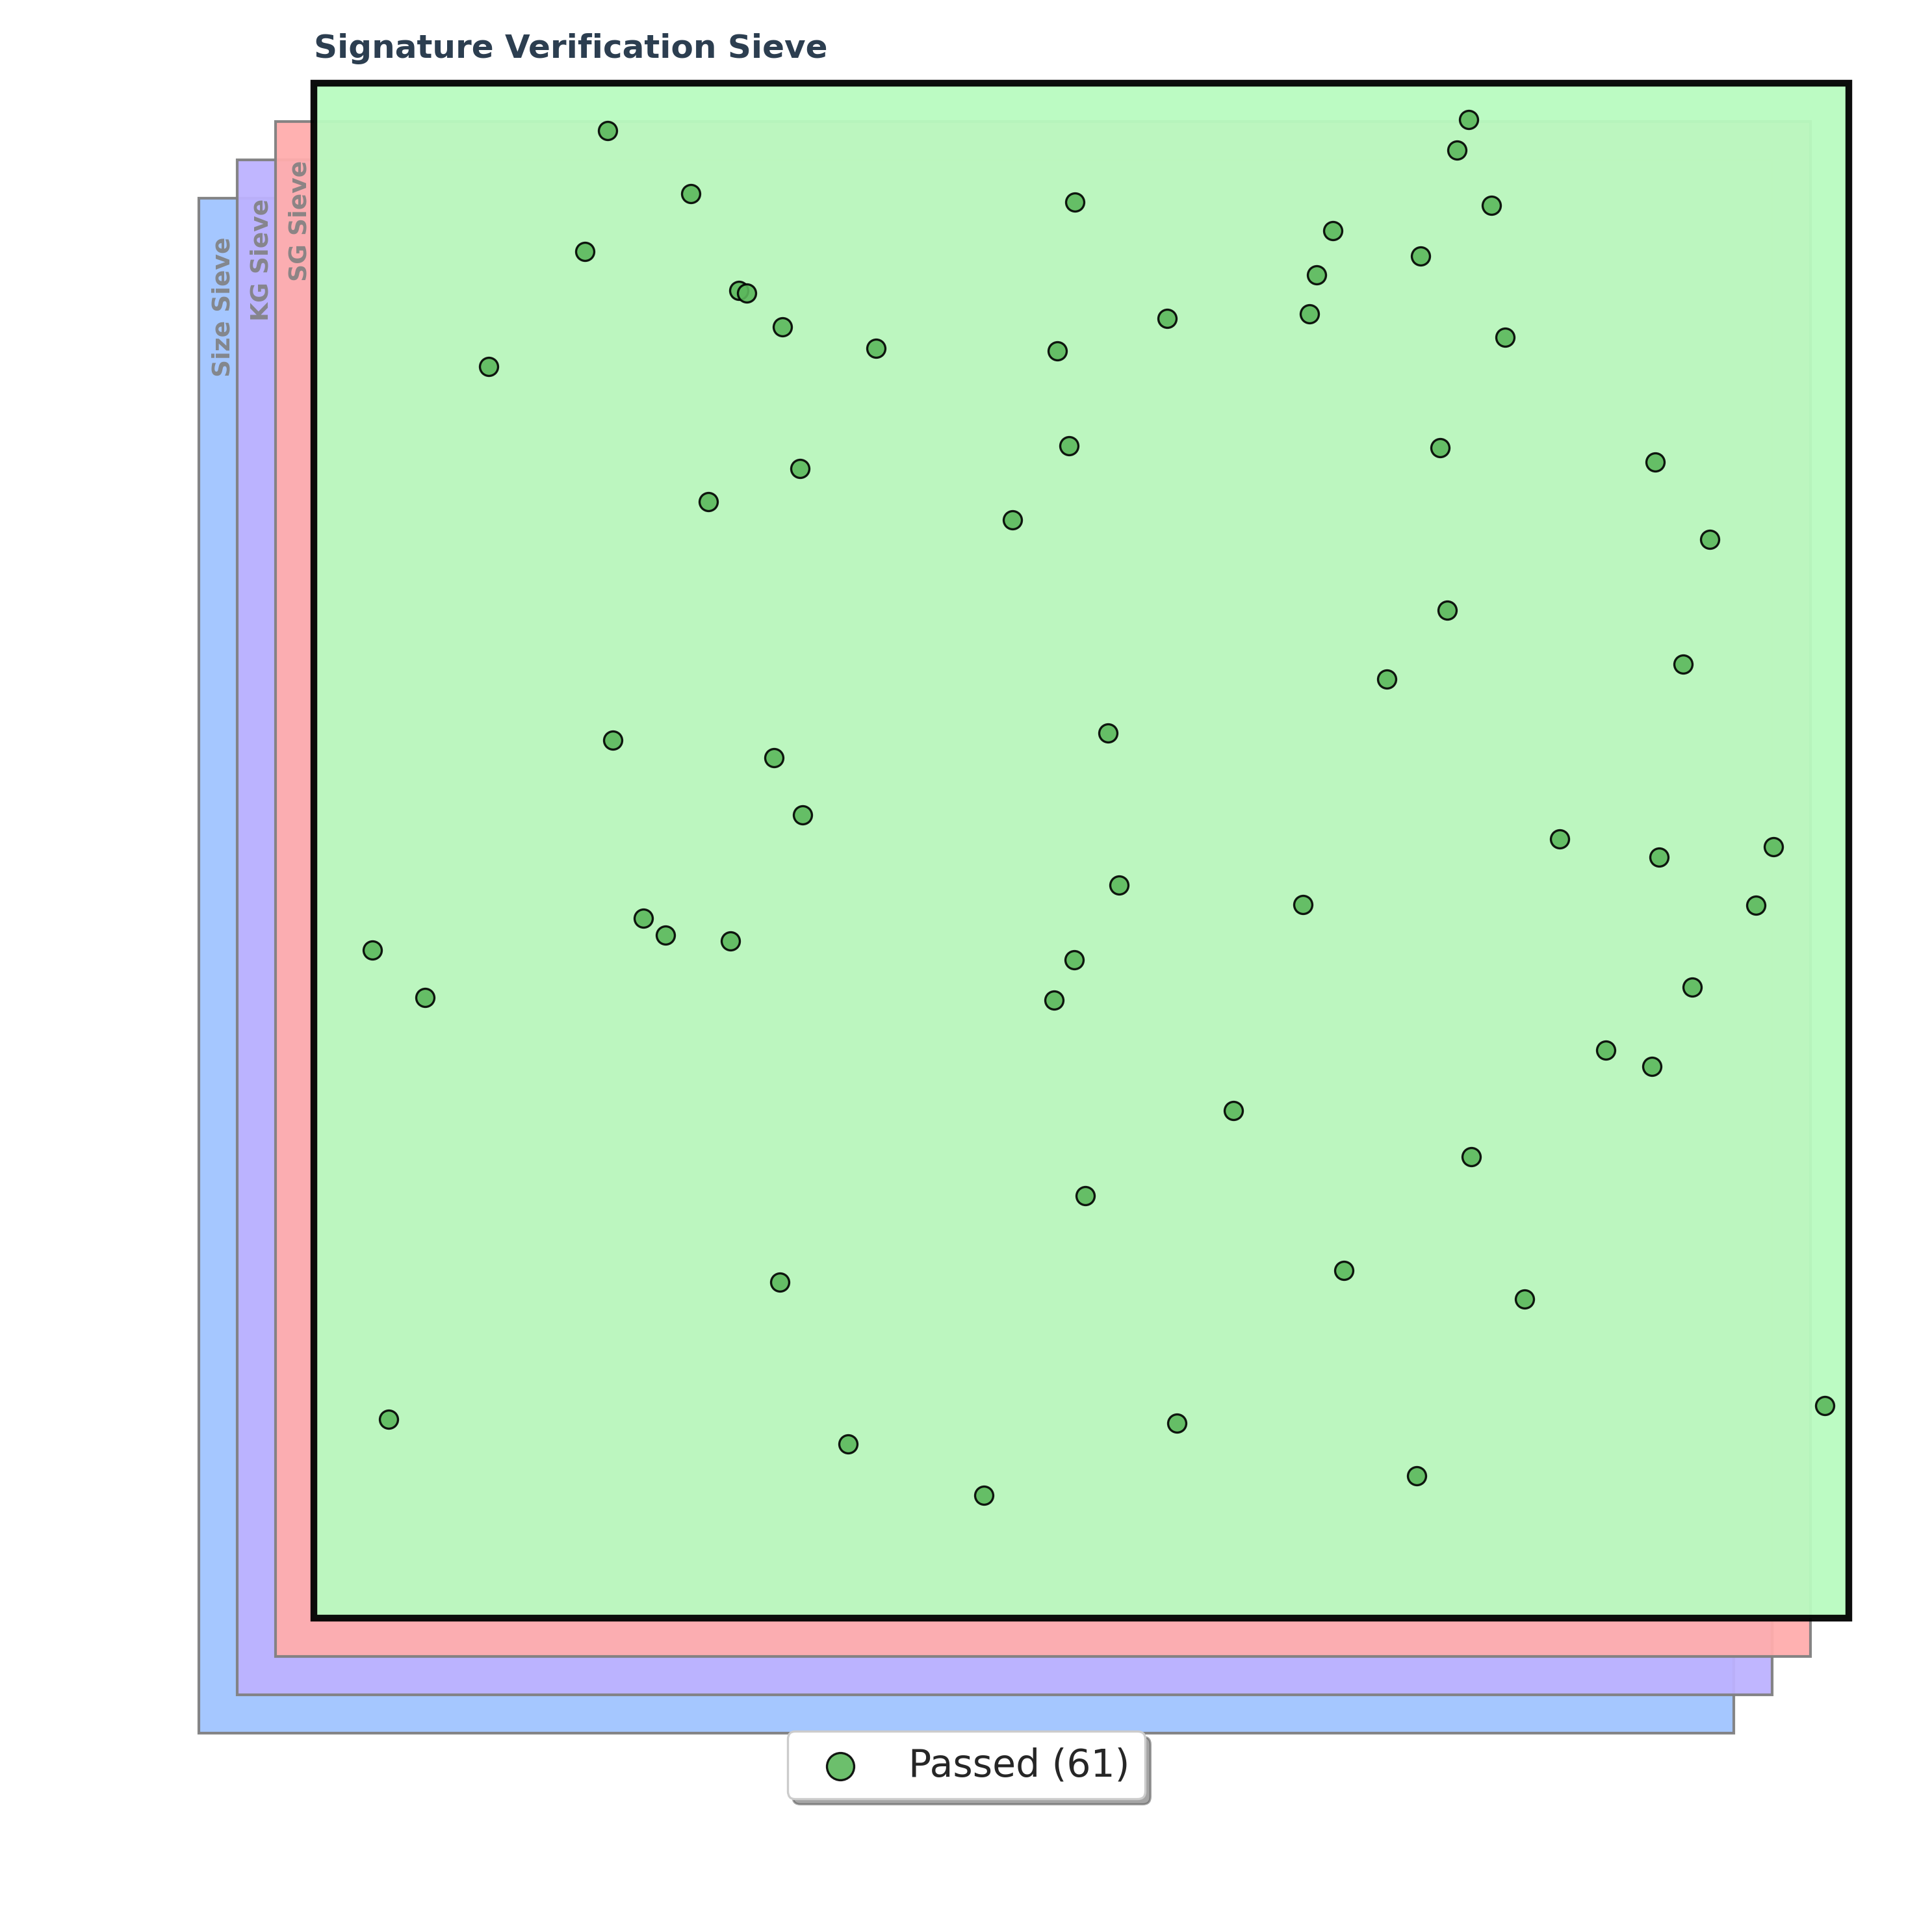
\includegraphics[width=\textwidth]{content/images/sieve_step5_verify.png}
        \caption{SigVerify}
        \label{fig:sieve_5}
    \end{subfigure}
    \hfill
    \begin{subfigure}[b]{0.32\textwidth}
        \centering
        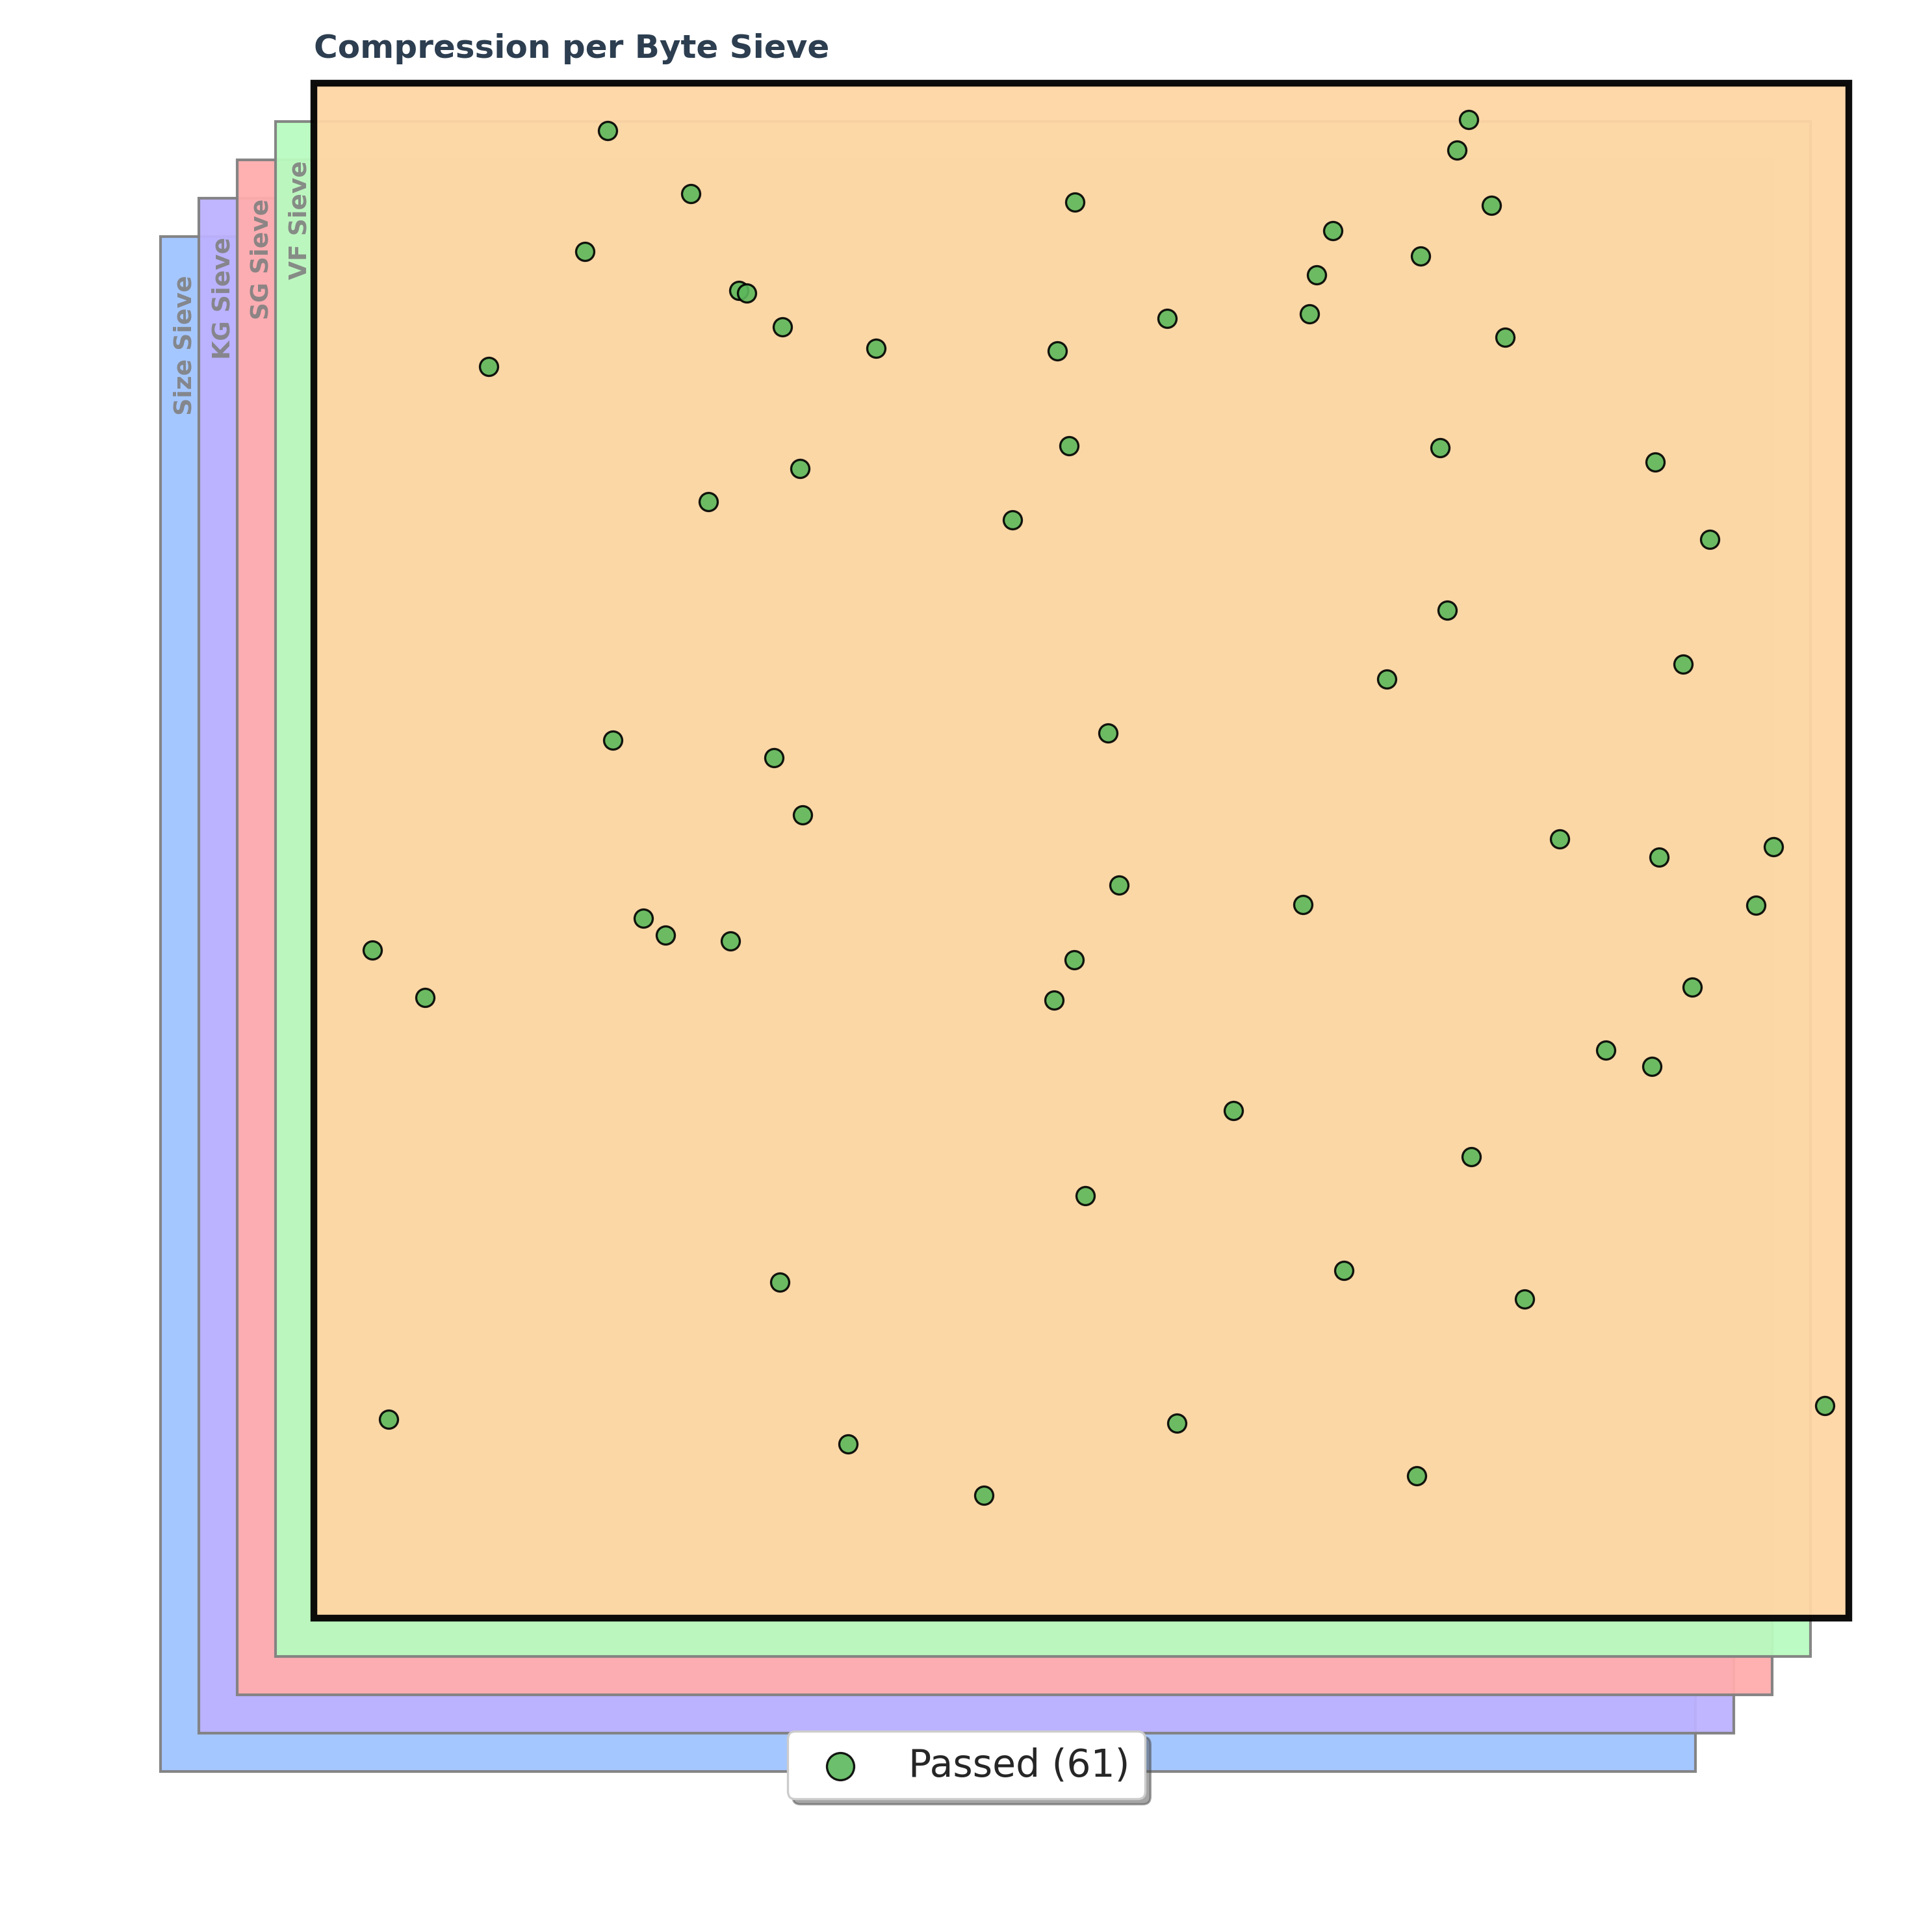
\includegraphics[width=\textwidth]{content/images/sieve_step6_rho.png}
        \caption{Comp/Byte}
        \label{fig:sieve_6}
    \end{subfigure}
    
    \caption{Full Parameter Filtering Process}
    \label{fig:full_filtering_process}
\end{figure}

We start with \emph{19,437} candidates. The signature-size filter trims the pool to \emph{6,202}; the next filter (KeyGen) cuts it by more than $7\times$. Each subsequent filter prunes further, leaving \emph{60} final candidates for inspection.

With the final 60 candidates in hand, we are ready to pick a winner.

For each surviving candidate $P$, let $\widetilde{X}_i$ denote the ratio of the candidate's value for metric $i$ to the corresponding standard value, where $i \in \{\text{size}, \text{kg}, \text{sg}, \text{sv}, \text{cb}\}$. Working with ratios rather than raw values keeps the five axes on a common, dimensionless scale. The Euclidean distance from the origin to $P$ is then
\begin{equation}
    d(P) = \sqrt{\widetilde{X}_{\text{size}}^2 + \widetilde{X}_{\text{kg}}^2 + \widetilde{X}_{\text{sg}}^2 + \widetilde{X}_{\text{sv}}^2 + \widetilde{X}_{\text{cb}}^2}\,,
    \label{eq:euclidean_distance}
\end{equation}
and the optimal candidate is the one minimizing $d(P)$.

This treats every metric as equally important, which is rarely what we actually want. Signature size, for example, usually carries far more weight than key-generation cost in a Bitcoin context. The next subsection addresses this by attaching weights to each axis.

\subsection{Decisional Weights} \label{sec:decisional-weights}
We can do better by applying the \emph{weighted} Euclidean distance. The motivation is that weights give us a principled way to encode the relative priority of each metric. Let $w_{\text{size}}, w_{\text{kg}}, w_{\text{sg}}, w_{\text{sv}}, w_{\text{cb}} \in \mathbb{R}^+$ denote the raw weight coefficients representing the relative importance of signature size, key generation, signing, verification, and compressions per byte, respectively.

To keep the calculation proportionally consistent regardless of the absolute scale of the chosen weights, we normalize them into coefficients $p_i$ (where $i \in \{\text{size}, \text{kg}, \text{sg}, \text{sv}, \text{cb}\}$) such that they sum to $1$:
\begin{equation}
    p_i = \frac{w_i}{w_{\text{size}} + w_{\text{kg}} + w_{\text{sg}} + w_{\text{sv}} + w_{\text{cb}}}, \quad \text{ensuring} \quad \sum p_i = 1
    \label{eq:weight_normalization}
\end{equation}

Using these normalized coefficients, we calculate the Weighted Euclidean Distance (the $L_2$ norm) from the origin $(0,0,0,0,0)$ to the candidate's point $P$. The distance $d(P)$ is defined as:
\begin{equation}
    d(P) = \sqrt{p_{\text{size}} \widetilde{X}_{\text{size}}^2 + p_{\text{kg}} \widetilde{X}_{\text{kg}}^2 + p_{\text{sg}} \widetilde{X}_{\text{sg}}^2 + p_{\text{sv}} \widetilde{X}_{\text{sv}}^2 + p_{\text{cb}} \widetilde{X}_{\text{cb}}^2}
    \label{eq:weighted_euclidean_distance}
\end{equation}

As before, each $\widetilde{X}_i$ is the ratio of the candidate's metric to its standard counterpart, so the five axes remain on a common dimensionless scale.

To visualize the distances, we map each candidate's distance onto a colour scale: lower distances shade towards blue, higher distances towards red. As an example, consider the following two weight settings:
\begin{itemize}
    \item Case 1: $w_{\text{size}} = w_{\text{kg}} = w_{\text{sg}} = w_{\text{sv}} = w_{\text{cb}} = 1$;
    \item Case 2: $w_{\text{size}} = 5,\ w_{\text{kg}} = 1,\ w_{\text{sg}} = 1.5,\ w_{\text{sv}} = 2,\ w_{\text{cb}} = 1$.
\end{itemize}

The result for the first case is shown below.

\begin{figure}[htbp]
    \centering
    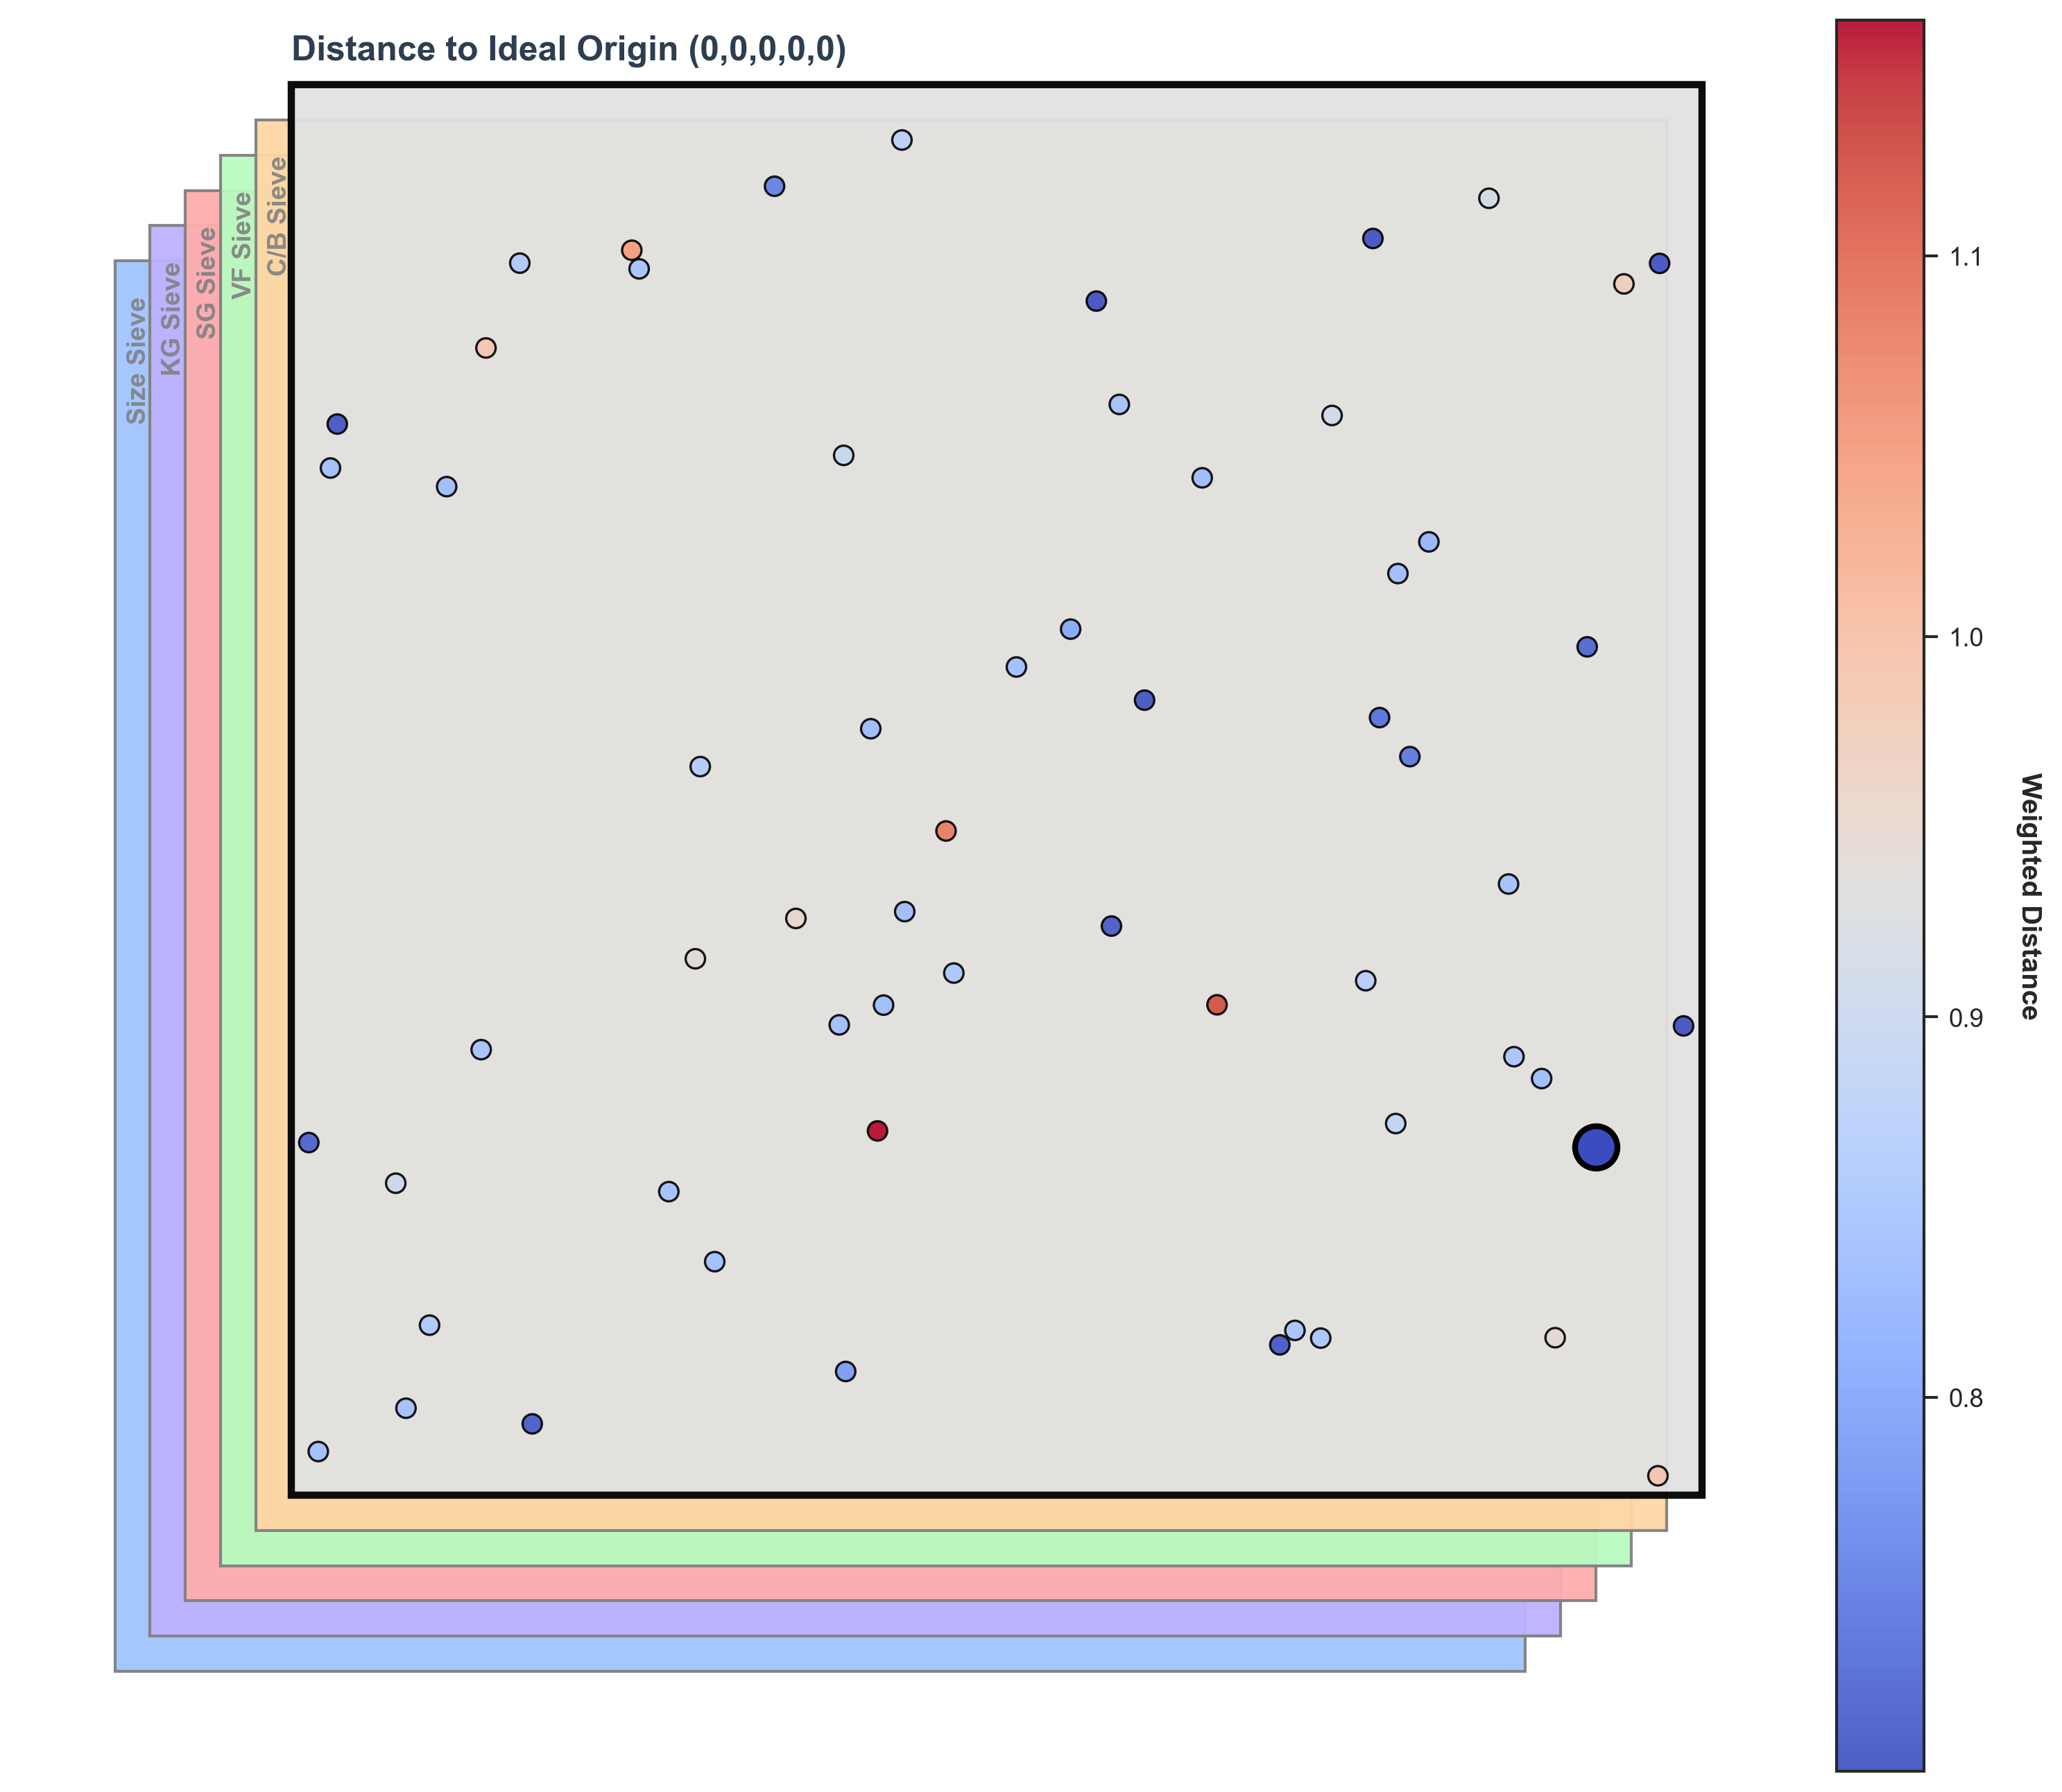
\includegraphics[width=0.75\textwidth]{content/images/sieve_step7_distance_1.png}
    \caption{Visualization of Searching for the Case 1.}
    \label{fig:distance_plot_1}
\end{figure}

The parameters and metric values of the best candidate are shown in Table~\ref{tab:euclidean_candidate_metrics_case_1}.


\begin{table}[htbp]
    \centering
    \small
    \caption{Performance Comparison between the Standard Baseline and the Best Shortest Distance Candidate}
    \label{tab:euclidean_candidate_metrics_case_1}
    \begin{tabular}{lrrr}
        \toprule
        \textbf{Metric} & \textbf{Standard Baseline} & \textbf{Best Candidate} & \textbf{Ratio to Std.} \\
        \midrule
        Parameters $(h, d, k, a, w)$ & $(63, 7, 14, 12, 16)$ & $(40, 5, 19, 9, 16)$ & -- \\
        Signature Size (Bytes) & $7,856$ & $6,496$ & $0.8269\times$ \\
        Key Generation Cost & $292,862$ & $146,430$ & $0.5000\times$ \\
        Signing Cost & $2,279,391$ & $771,034$ & $0.3383\times$ \\
        Verification Cost & $2,387$ & $1,809$ & $0.7579\times$ \\
        Compression per Byte ($\rho$) & $0.3038$ & $0.2785$ & $0.9167\times$ \\
        \bottomrule
    \end{tabular}
\end{table}

\newpage

For the second case, we have the following picture:

\begin{figure}[htbp]
    \centering
    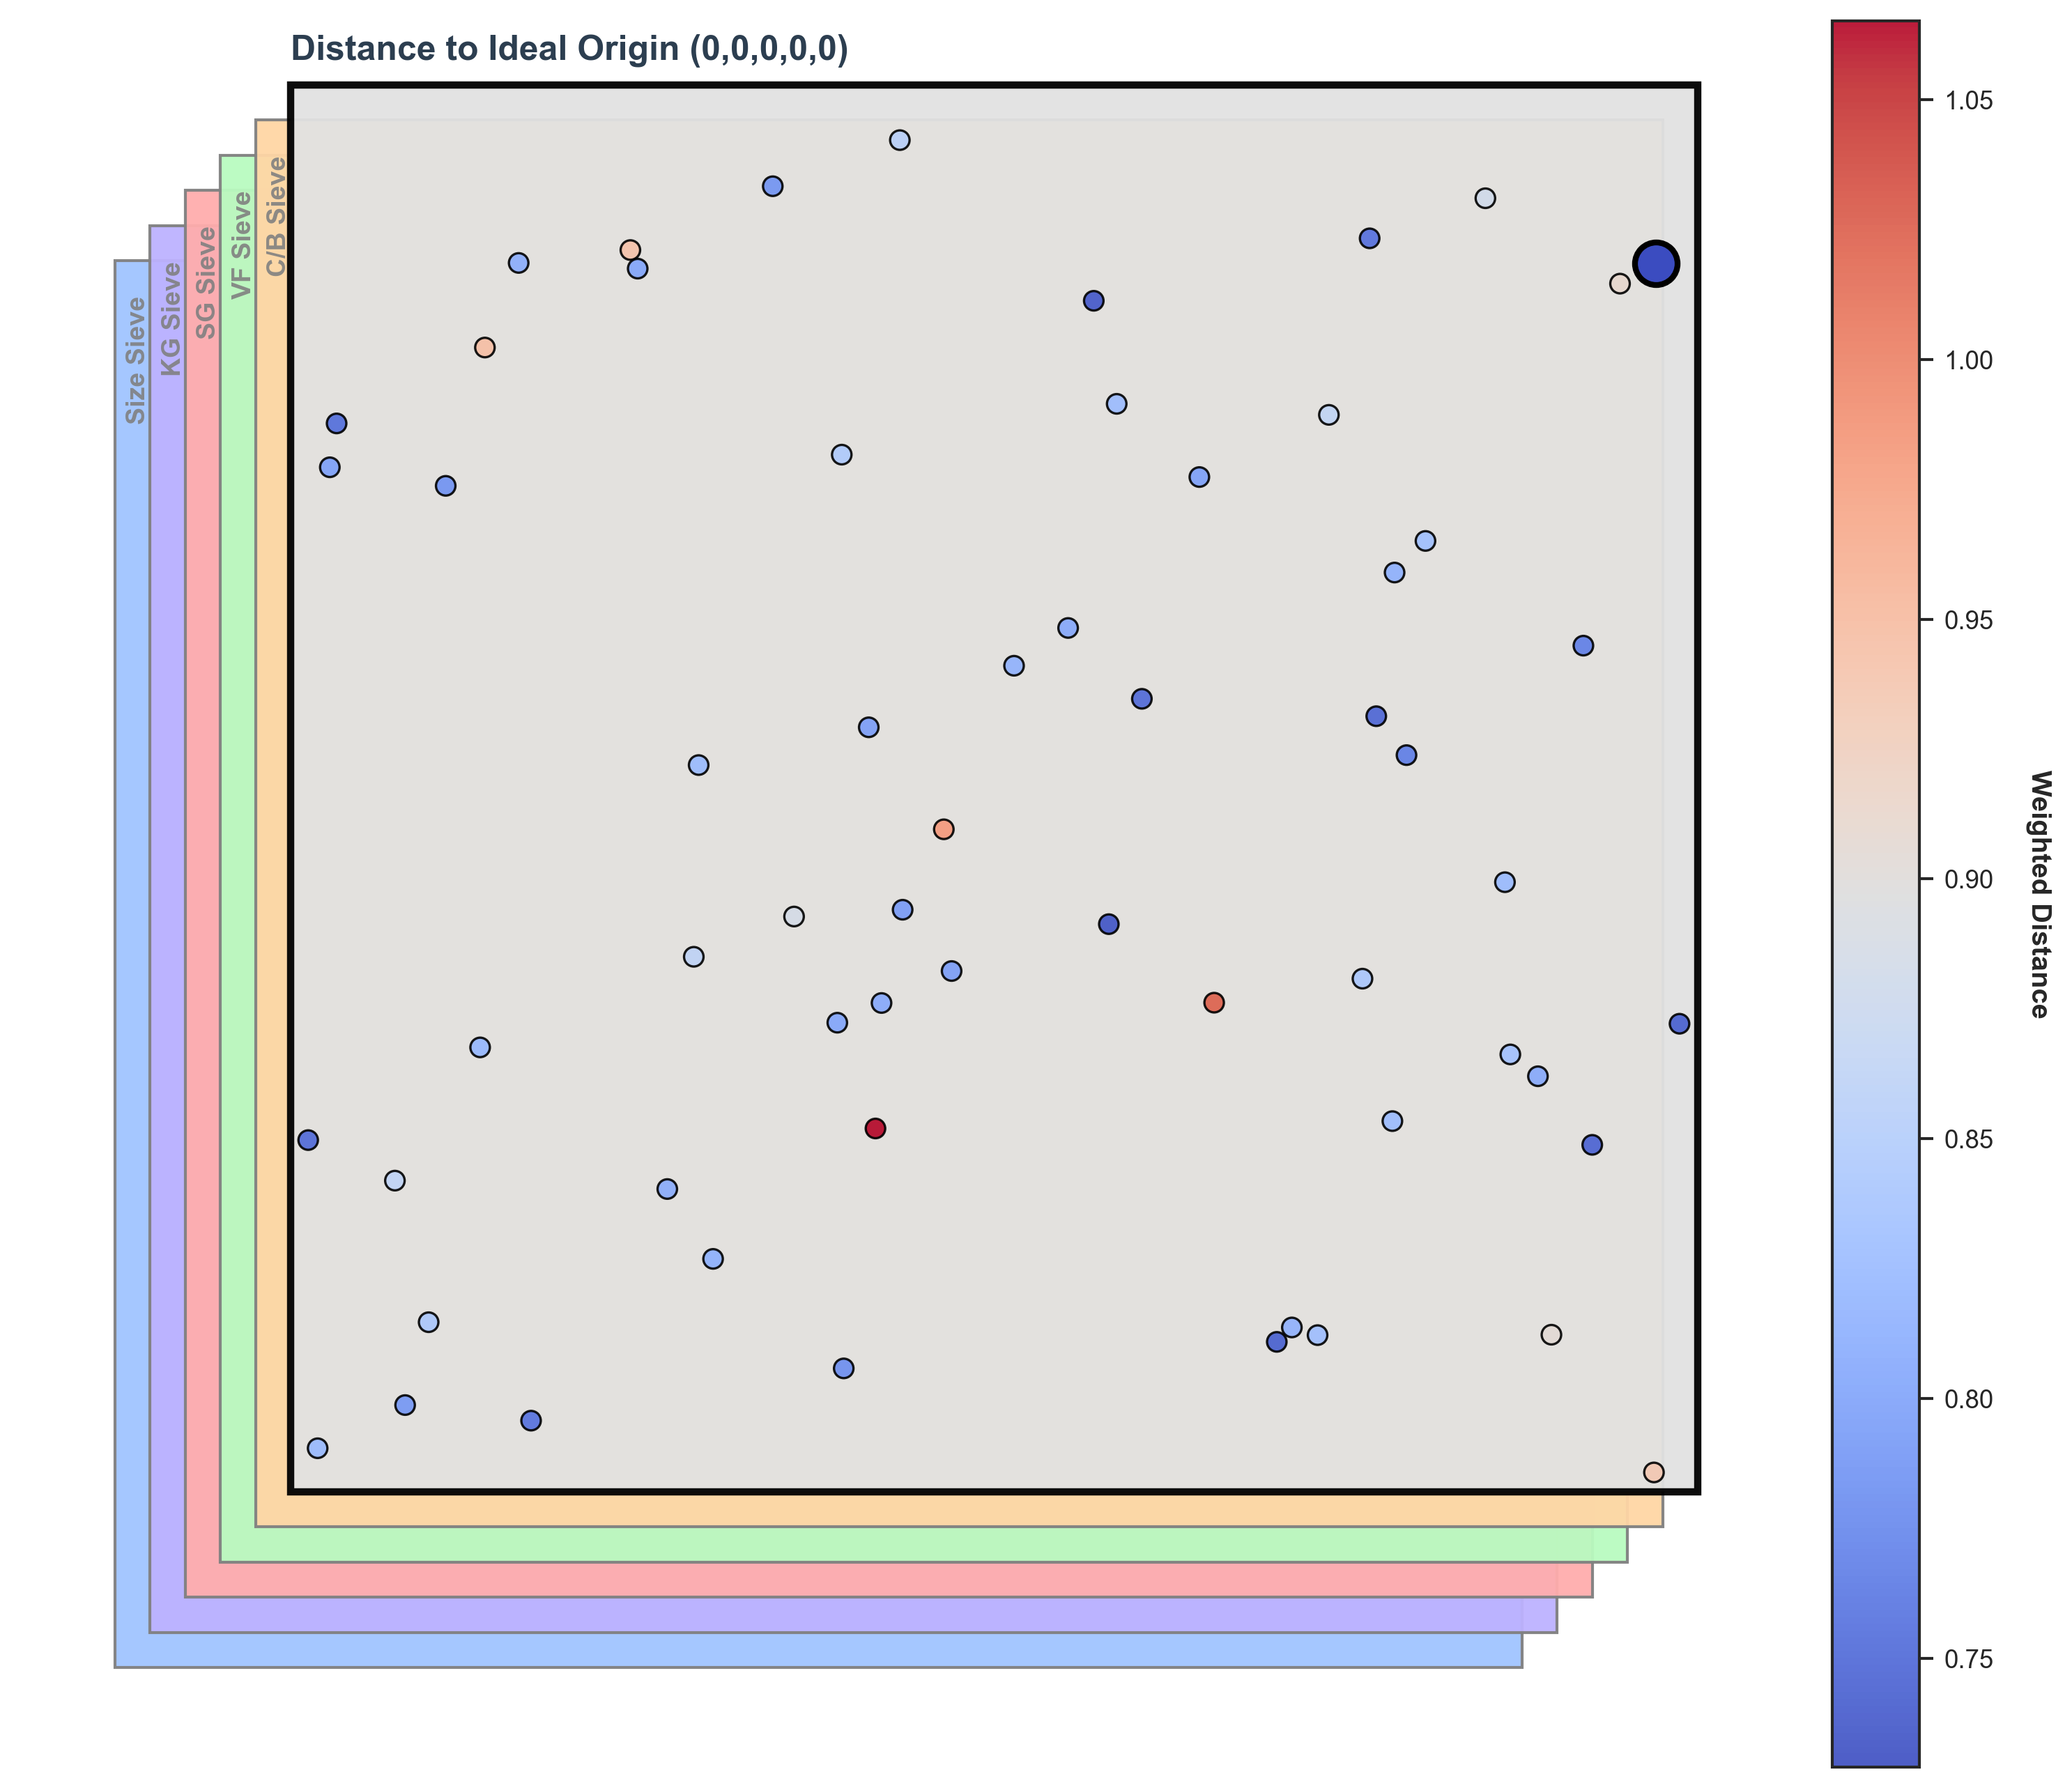
\includegraphics[width=0.75\textwidth]{content/images/sieve_step7_distance_2.png}
    \caption{Visualization of Searching for the Case 2.}
    \label{fig:distance_plot_2}
\end{figure}

The resulting values are shown in Table~\ref{tab:euclidean_candidate_metrics_case_2}.

\begin{table}[htbp]
    \centering
    \small
    \caption{Performance Comparison between the Standard Baseline and the Best Shortest Distance Candidate}
    \label{tab:euclidean_candidate_metrics_case_2}
    \begin{tabular}{lrrr}
        \toprule
        \textbf{Metric} & \textbf{Standard Baseline} & \textbf{Best Candidate} & \textbf{Ratio to Std.} \\
        \midrule
        Parameters $(h, d, k, a, w)$ & $(63, 7, 14, 12, 16)$ & $(40, 5, 13, 12, 16)$ & -- \\
        Signature Size (Bytes) & $7,856$ & $6,160$ & $0.7841\times$ \\
        Key Generation Cost & $292,862$ & $146,430$ & $0.5000\times$ \\
        Signing Cost & $2,279,391.0$ & $945,124$ & $0.4146\times$ \\
        Verification Cost & $2,387.0$ & $1,771$ & $0.7419\times$ \\
        Compression per Byte ($\rho$) & $0.3038$ & $0.2875$ & $0.9463\times$ \\
        \bottomrule
    \end{tabular}
\end{table}

Comparing the two cases, the resulting metrics differ noticeably. The first case yields more balanced costs across the board, while the second case clearly favours signature size and verification at the expense of a heavier signing operation - exactly the trade-off we asked the weights to enforce. 

\subsection{Metric-Normalized Weighted Distance} \label{sec:normalized-weights}

The weighted distance introduced in Section~\ref{sec:decisional-weights} correctly encodes relative priorities when the five ratio axes $\widetilde{X}_i$ vary over comparable ranges.
In practice, however, the filter pipeline disturbs this assumption.
Consider the signature-size filter: after it is applied with a tight coefficient $X_{\text{size}} \ll 1$, every surviving candidate has a ratio $\widetilde{X}_{\text{size}}$ that lies in a narrow band close to $X_{\text{size}}$.
The range of $\widetilde{X}_{\text{size}}$ values across survivors is therefore small relative to the variation of cost metrics such as $\widetilde{X}_{\text{kg}}$ or $\widetilde{X}_{\text{sg}}$, which the filter may leave nearly unconstrained.
As a result, the size term contributes almost the same value to $d(P)$ for every candidate in the pool, regardless of the weight $p_{\text{size}}$ attached to it.
The ranking is then dominated by the high-variance axes, and increasing $w_{\text{size}}$ produces little to no change in which candidate is selected.

The remedy is to remove the scale imbalance before applying the weights.
For each metric $i$ and each surviving candidate $P_j$ in the current pool, define the cross-pool minimum and maximum of the ratios:

\begin{equation}
    m_i = \min_j \widetilde{X}_i(P_j), \qquad
    M_i = \max_j \widetilde{X}_i(P_j).
    \label{eq:metric_range}
\end{equation}

The \emph{metric-normalized ratio} of candidate $P$ on axis $i$ is then

\begin{equation}
    \widehat{X}_i(P) = \frac{\widetilde{X}_i(P) - m_i}{M_i - m_i},
    \label{eq:metric_norm}
\end{equation}

which maps every axis to $[0, 1]$ across the survivor pool, with $\widehat{X}_i = 0$ identifying the best-performing candidate on that axis and $\widehat{X}_i = 1$ the worst-performing one.

Replacing $\widetilde{X}_i$ with $\widehat{X}_i$ in Equation~\eqref{eq:weighted_euclidean_distance} yields the \emph{metric-normalized weighted Euclidean distance}:

\begin{equation}
    d(P) = \sqrt{
        p_{\text{size}}\,\widehat{X}_{\text{size}}^2 +
        p_{\text{kg}}\,\widehat{X}_{\text{kg}}^2 +
        p_{\text{sg}}\,\widehat{X}_{\text{sg}}^2 +
        p_{\text{sv}}\,\widehat{X}_{\text{sv}}^2 +
        p_{\text{cb}}\,\widehat{X}_{\text{cb}}^2
    },
    \label{eq:normalized_weighted_distance}
\end{equation}

where the $p_i$ are the normalized weight coefficients from Equation~\eqref{eq:weight_normalization}.
The winner is still the candidate minimising $d(P)$, but now the weight $p_i$ faithfully controls how much axis $i$ influences the ranking: because every $\widehat{X}_i$ spans the same $[0, 1]$ interval, a coefficient $p_{\text{size}} = 0.5$ means that signature size drives exactly half of the squared distance, independently of how tightly the size filter was set.

\paragraph{Note:}
The normalization is computed fresh from the survivors after each change to the filter coefficients.
This means that the same weight vector $\mathbf{w}$ can produce a different winner when the filter is tightened, because the pool shrinks and the per-axis ranges change accordingly.
This behaviour is intentional: the weights express relative importance \emph{within the feasible region}, and that region is itself defined by the filter.

Consider the following filtering parameters and weights set for comparison of methods for finding the shortest vector with weights: 

\begin{itemize}
    \item Filtering parameters: $X_{\text{size}} = 0.75, \ X_{\text{kg}} = 5, \ X_{\text{sg}} = 5, \ X_{\text{sv}} = 1.5, \ X_{\text{cb}} = 1$;
    \item Weights coefficients: $w_{\text{size}} = 5, \ w_{\text{kg}} = 1.5, \ w_{\text{sg}} = 1.5, \ w_{\text{sv}} = 2, \ w_{\text{cb}} = 1$.
\end{itemize}

The resulting best candidates for each method shown in the Table~\ref{tab:distance_method_comparison}.

\begin{table}[htbp]
\centering
\small
\raggedright
\caption{Comparison between the Best Candidates under the Regular Weighted and Metric-Normalised Weighted Distance Criteria}
\label{tab:distance_method_comparison}
\resizebox{\textwidth}{!}{%
\begin{tabular}{lrrrrr}
\toprule
\textbf{Metric} &
\textbf{Standard Baseline} &
\textbf{Metric-Normalized} &
\textbf{Ratio to Std.} &
\textbf{Regular Weighted} &
\textbf{Ratio to Std.} \\
\midrule
Parameters $(h, d, k, a, w)$  & $(63, 7, 14, 12, 16)$ & $(40, 4, 9, 16, 16)$  & --             & $(45, 5, 12, 11, 16)$ & --             \\
Signature Size (Bytes)        & $7{,}856$             & $5{,}344$             & $0.6802\times$ & $5{,}840$             & $0.7434\times$ \\
Key Generation Cost           & $292{,}862$           & $585{,}726$           & $2.0000\times$ & $292{,}862$           & $1.0000\times$ \\
Signing Cost                  & $2{,}279{,}391$       & $4{,}702{,}189$       & $2.0629\times$ & $1{,}562{,}598$       & $0.6855\times$ \\
Verification Cost             & $2{,}387$             & $1{,}470$             & $0.6158\times$ & $1{,}732$             & $0.7256\times$ \\
Compression per Byte ($\rho$) & $0.3038$            & $0.2750$            & $0.9053\times$ & $0.2965$            & $0.9761\times$ \\
\bottomrule
\end{tabular}%
}
\end{table}

Comparing the two cases, the resulting metrics are different.
The regular weighted distance chooses more balanced best candidate, while the metric-normilized weighted distance selects candidate with noticeably smaller signature size, trading the key and signature generation costs.

The outcome of each distance method shown in the Figure~\ref{fig:distance_result_comparison}.


\begin{figure}[h!]
    \centering
    \begin{subfigure}[b]{0.49\textwidth}
        \centering
        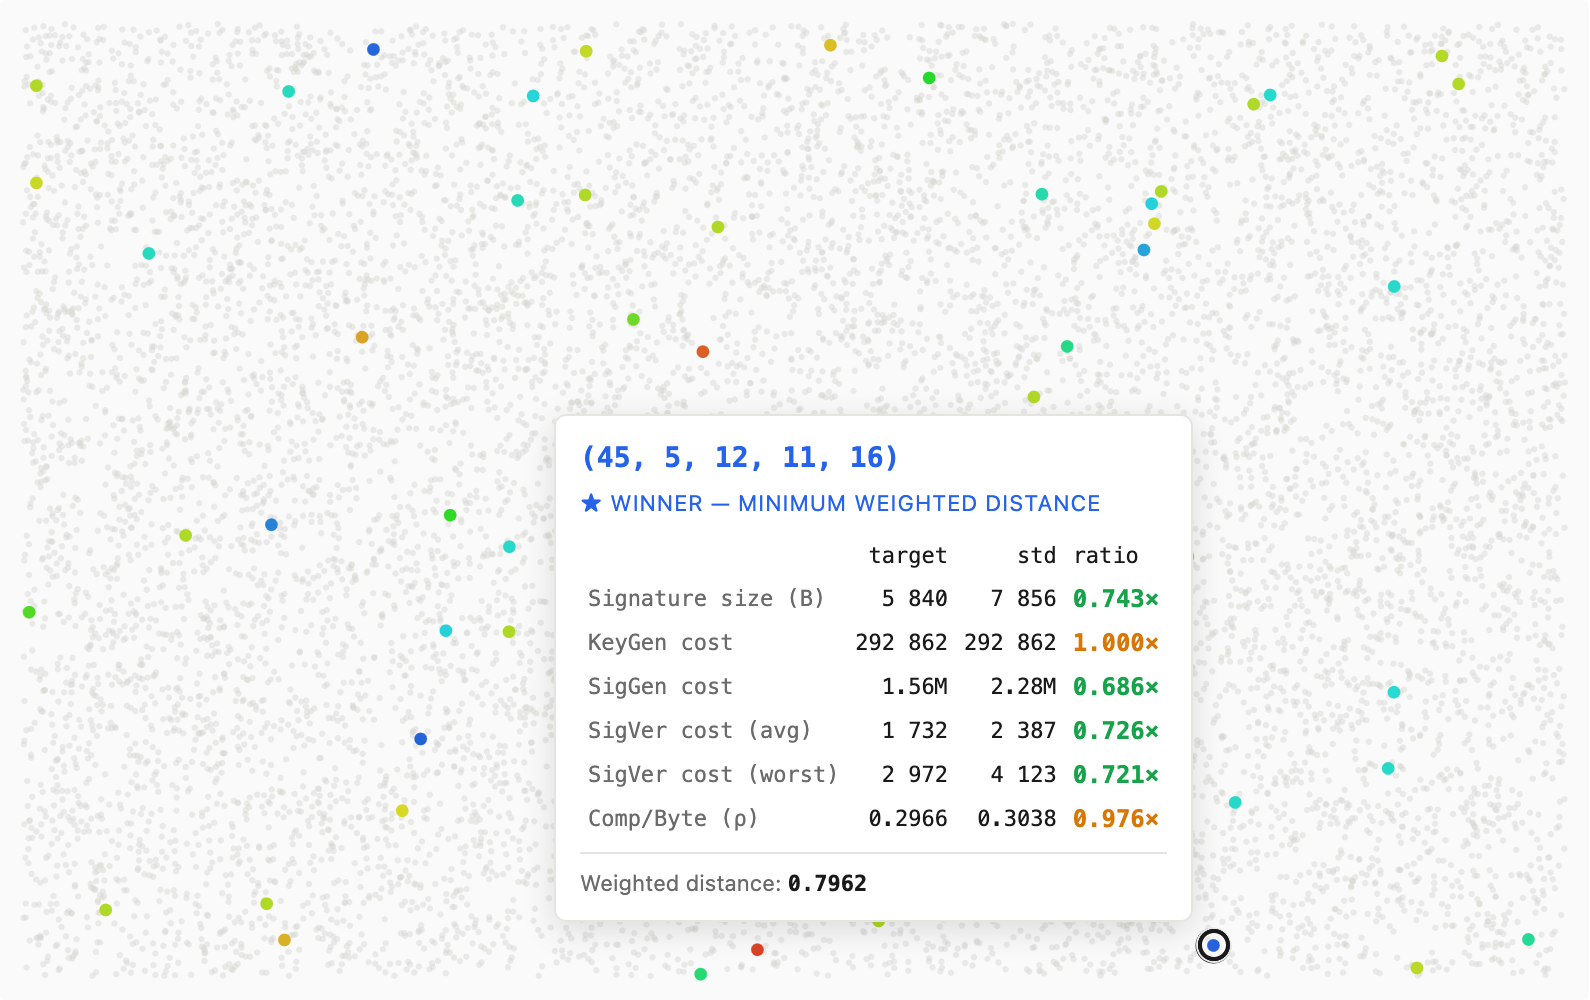
\includegraphics[width=\textwidth]{content/images/comparison_regular.png}
        \caption{Regular Weighted Distance Result}
        \label{fig:regular-weighted}
    \end{subfigure}
    \hfill
    \begin{subfigure}[b]{0.49\textwidth}
        \centering
        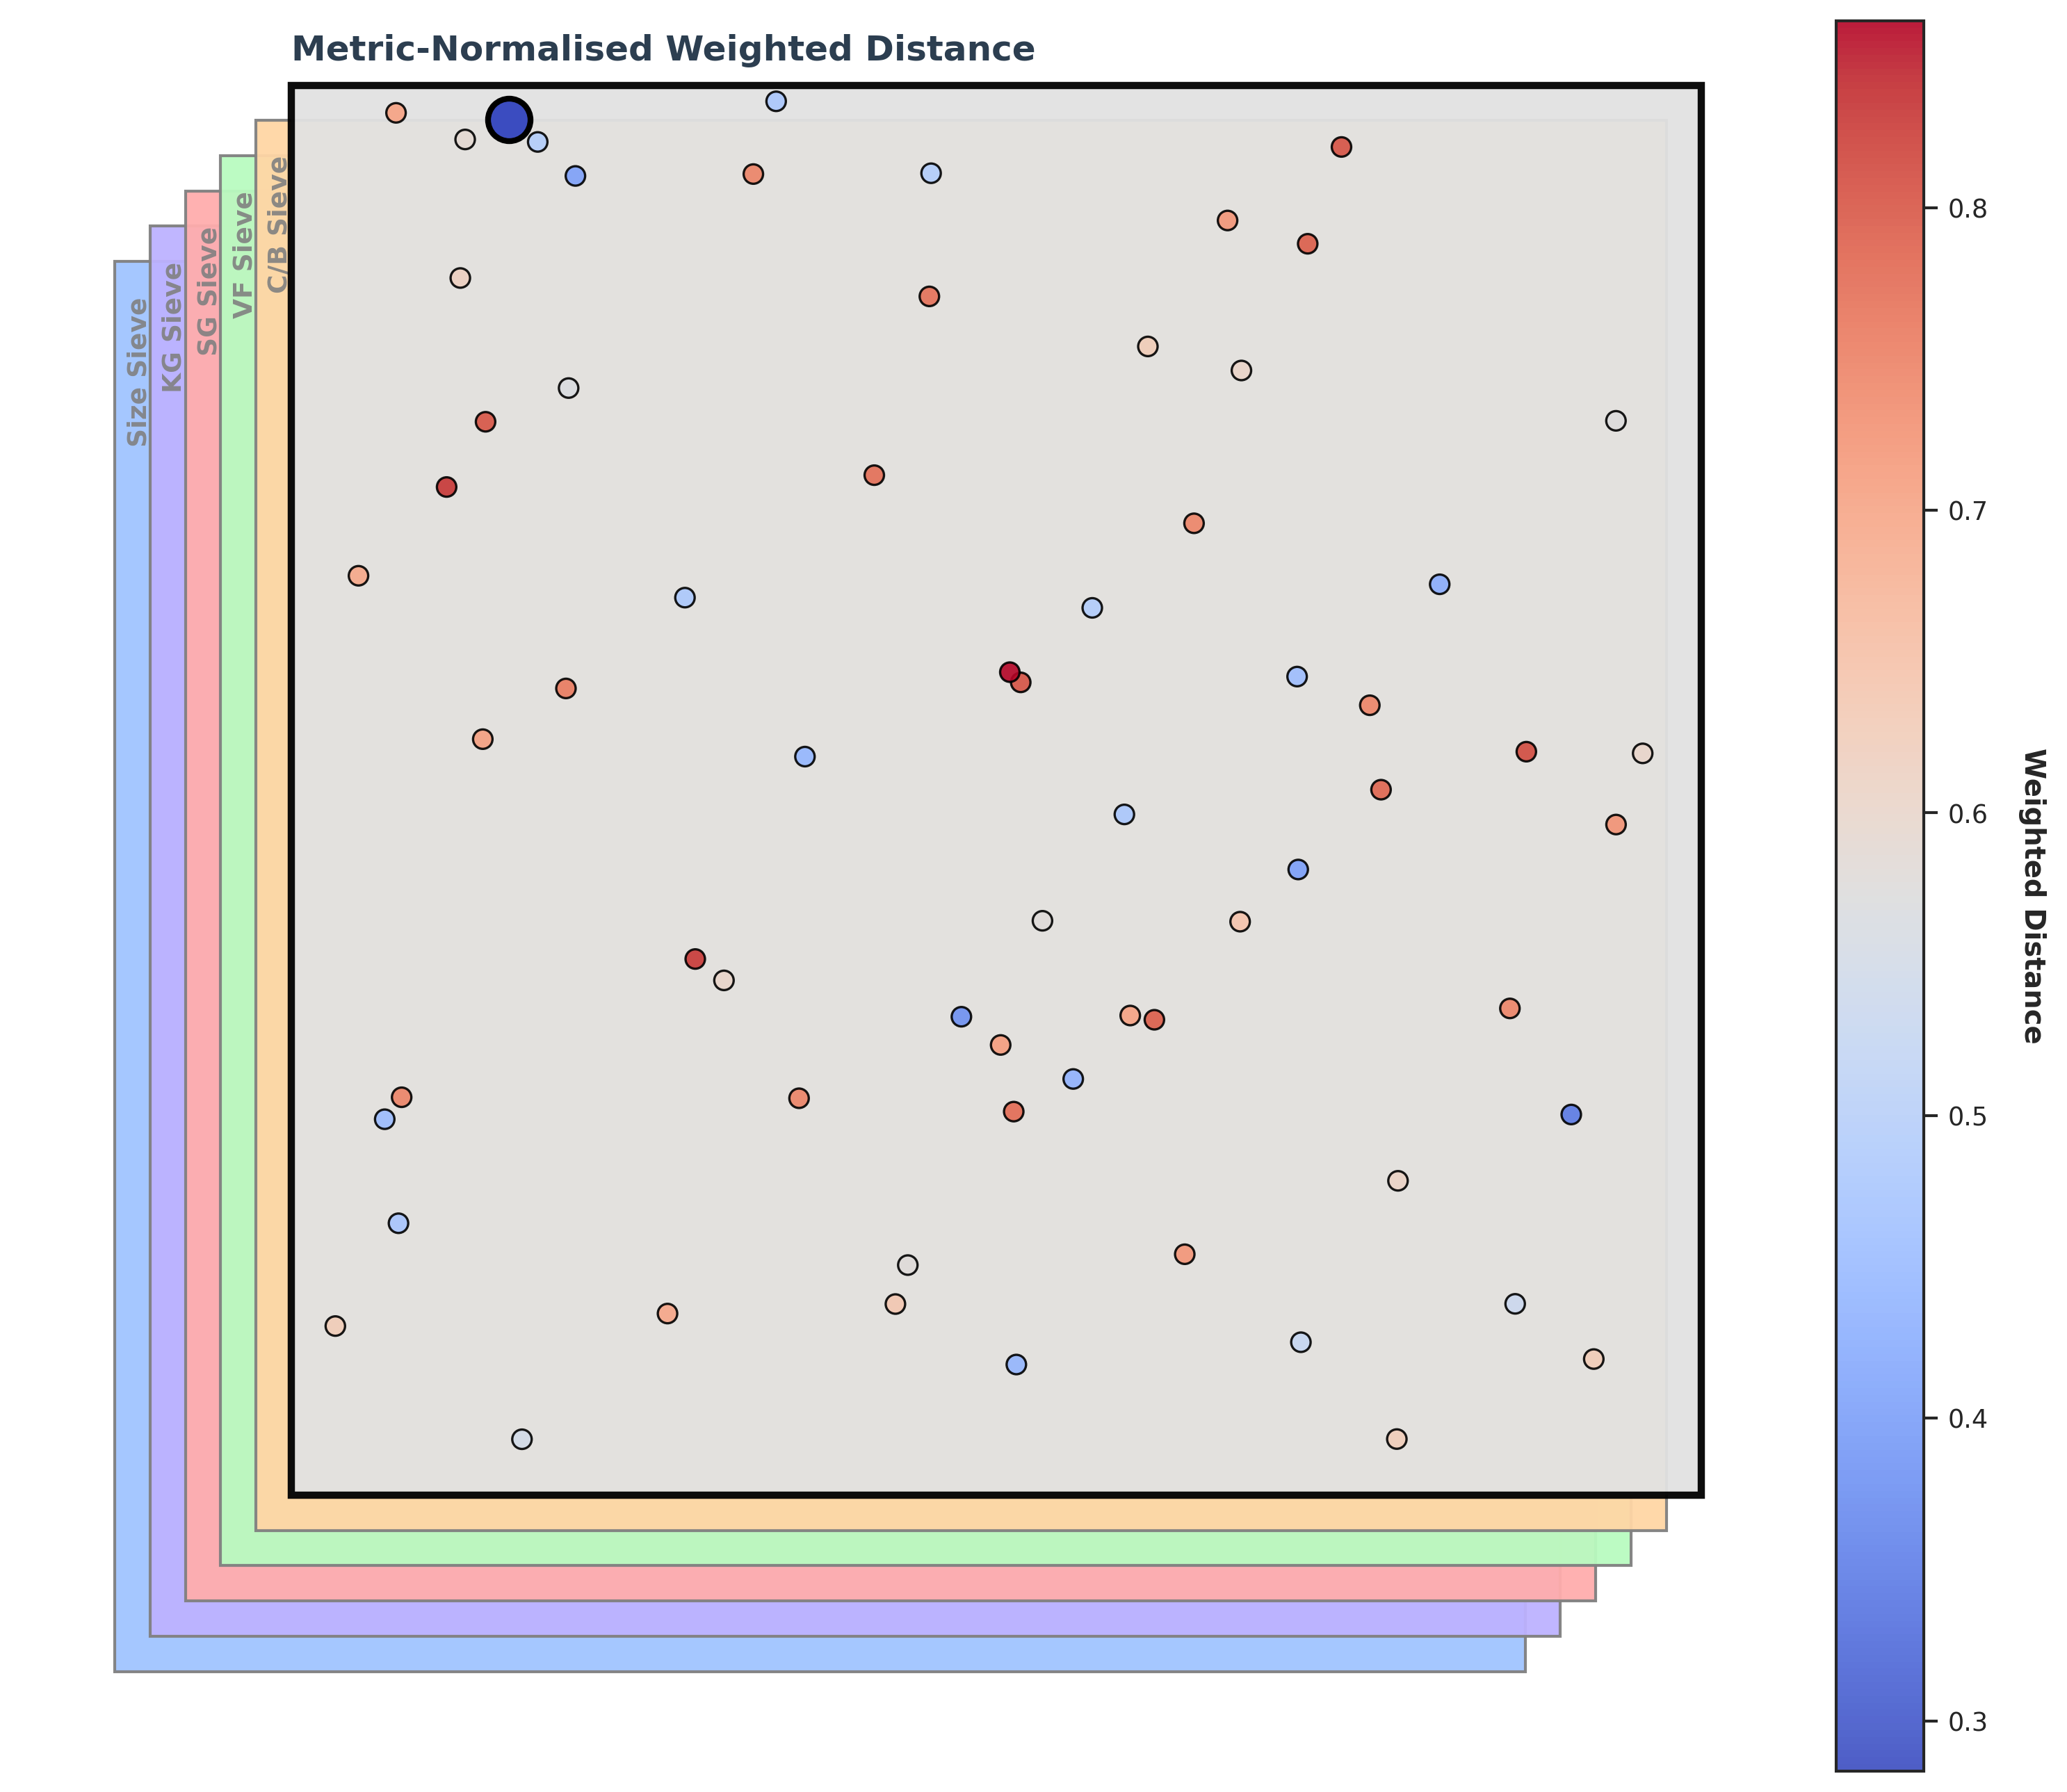
\includegraphics[width=\textwidth]{content/images/comparison_normalized.png}
        \caption{Metric-Normalised Weighted Distance Result}
        \label{fig:metric-normalised}
    \end{subfigure}
    \caption{Visualization of each Distance Method Result for Finding the Shortest Vector}
    \label{fig:distance_result_comparison}
\end{figure}



\section{Recommended Candidate Tuple} \label{sec:ideal-examples}

To demonstrate the full pipeline on a concrete parameter set we selected, we fix the following filtering coefficients:
\begin{equation*}
    X_{\text{size}} = 0.74, \quad X_{\text{kg}} = 2.0, \quad X_{\text{sg}} = 2.0,
    \quad X_{\text{sv}} = 0.8, \quad X_{\text{cb}} = 1.0.
\end{equation*}
These coefficients say that we really care about the signature size (to make at least 25\% win) and the verification complexity. At the same time having the key and signature complexity 2$\times$ at most is a acceptable trade-off because (1) it's not very critical taking into account even hardware wallet takes 2-3 seconds to produce SLH-DSA signature, (2) we can apply pruning technique \cite{conduition-blog} to reduce it additionally.  

Applying these constraints to the full parameter grid leaves exactly two surviving configurations, whose metrics are compared against the standard baseline in Table~\ref{tab:euclidean_candidate_metrics_ideal}.

\begin{table}[htbp]
\centering
\small
\raggedright
\caption{Performance Comparison between the Standard Baseline and the Two Evaluated Candidates}
\label{tab:euclidean_candidate_metrics_ideal}
\resizebox{\textwidth}{!}{%
\begin{tabular}{lrrrrr}
\toprule
\textbf{Metric} & \textbf{Standard Baseline} & \textbf{Candidate 1} &
\textbf{Ratio to Std.} & \textbf{Candidate 2} & \textbf{Ratio to Std.} \\
\midrule
Parameters $(h, d, k, a, w)$      & $(63, 7, 14, 12, 16)$ & $(45, 5, 10, 13, 16)$ & --             & $(45, 5, 8, 16, 16)$  & --             \\
Signature Size (Bytes)            & $7{,}856$             & $5{,}776$             & $0.7352\times$ & $5{,}712$             & $0.7271\times$ \\
Key Generation Cost               & $292{,}862$           & $292{,}862$           & $1.0000\times$ & $292{,}862$           & $1.0000\times$ \\
Signing Cost                      & $2{,}279{,}391$       & $1{,}791{,}978$       & $0.7862\times$ & $3{,}561{,}453$       & $1.5625\times$ \\
Verification Cost                 & $2{,}387$             & $1{,}726$             & $0.7231\times$ & $1{,}719$             & $0.7202\times$ \\
Compression per Byte ($\rho$)     & $0.3038$            & $0.2988$            & $0.9835\times$ & $0.3009$            & $0.9905\times$ \\
\bottomrule
\end{tabular}
}
\end{table}

As the table makes clear, the two survivors represent distinct operational trade-offs.
\begin{itemize}
    \item Candidate~1 offers a well-rounded improvement: signature size, signing cost, and verification cost all decrease relative to the standard.
    \item Candidate~2 pushes further on size and verification, but at a concrete price - its signing cost exceeds the standard by more than $1.5\times$, making it suitable only in contexts where signing latency is secondary.
\end{itemize}

Regardless of the weights that prioritizes size and verification cost, we get that the Candidate~1 is the best, having the smallest distance. 
The results of the search presented in the Figure~\ref{fig:ideal_distance_plot}.
\begin{figure}[htbp]
\centering
    \begin{subfigure}[b]{0.49\textwidth}
        \centering
        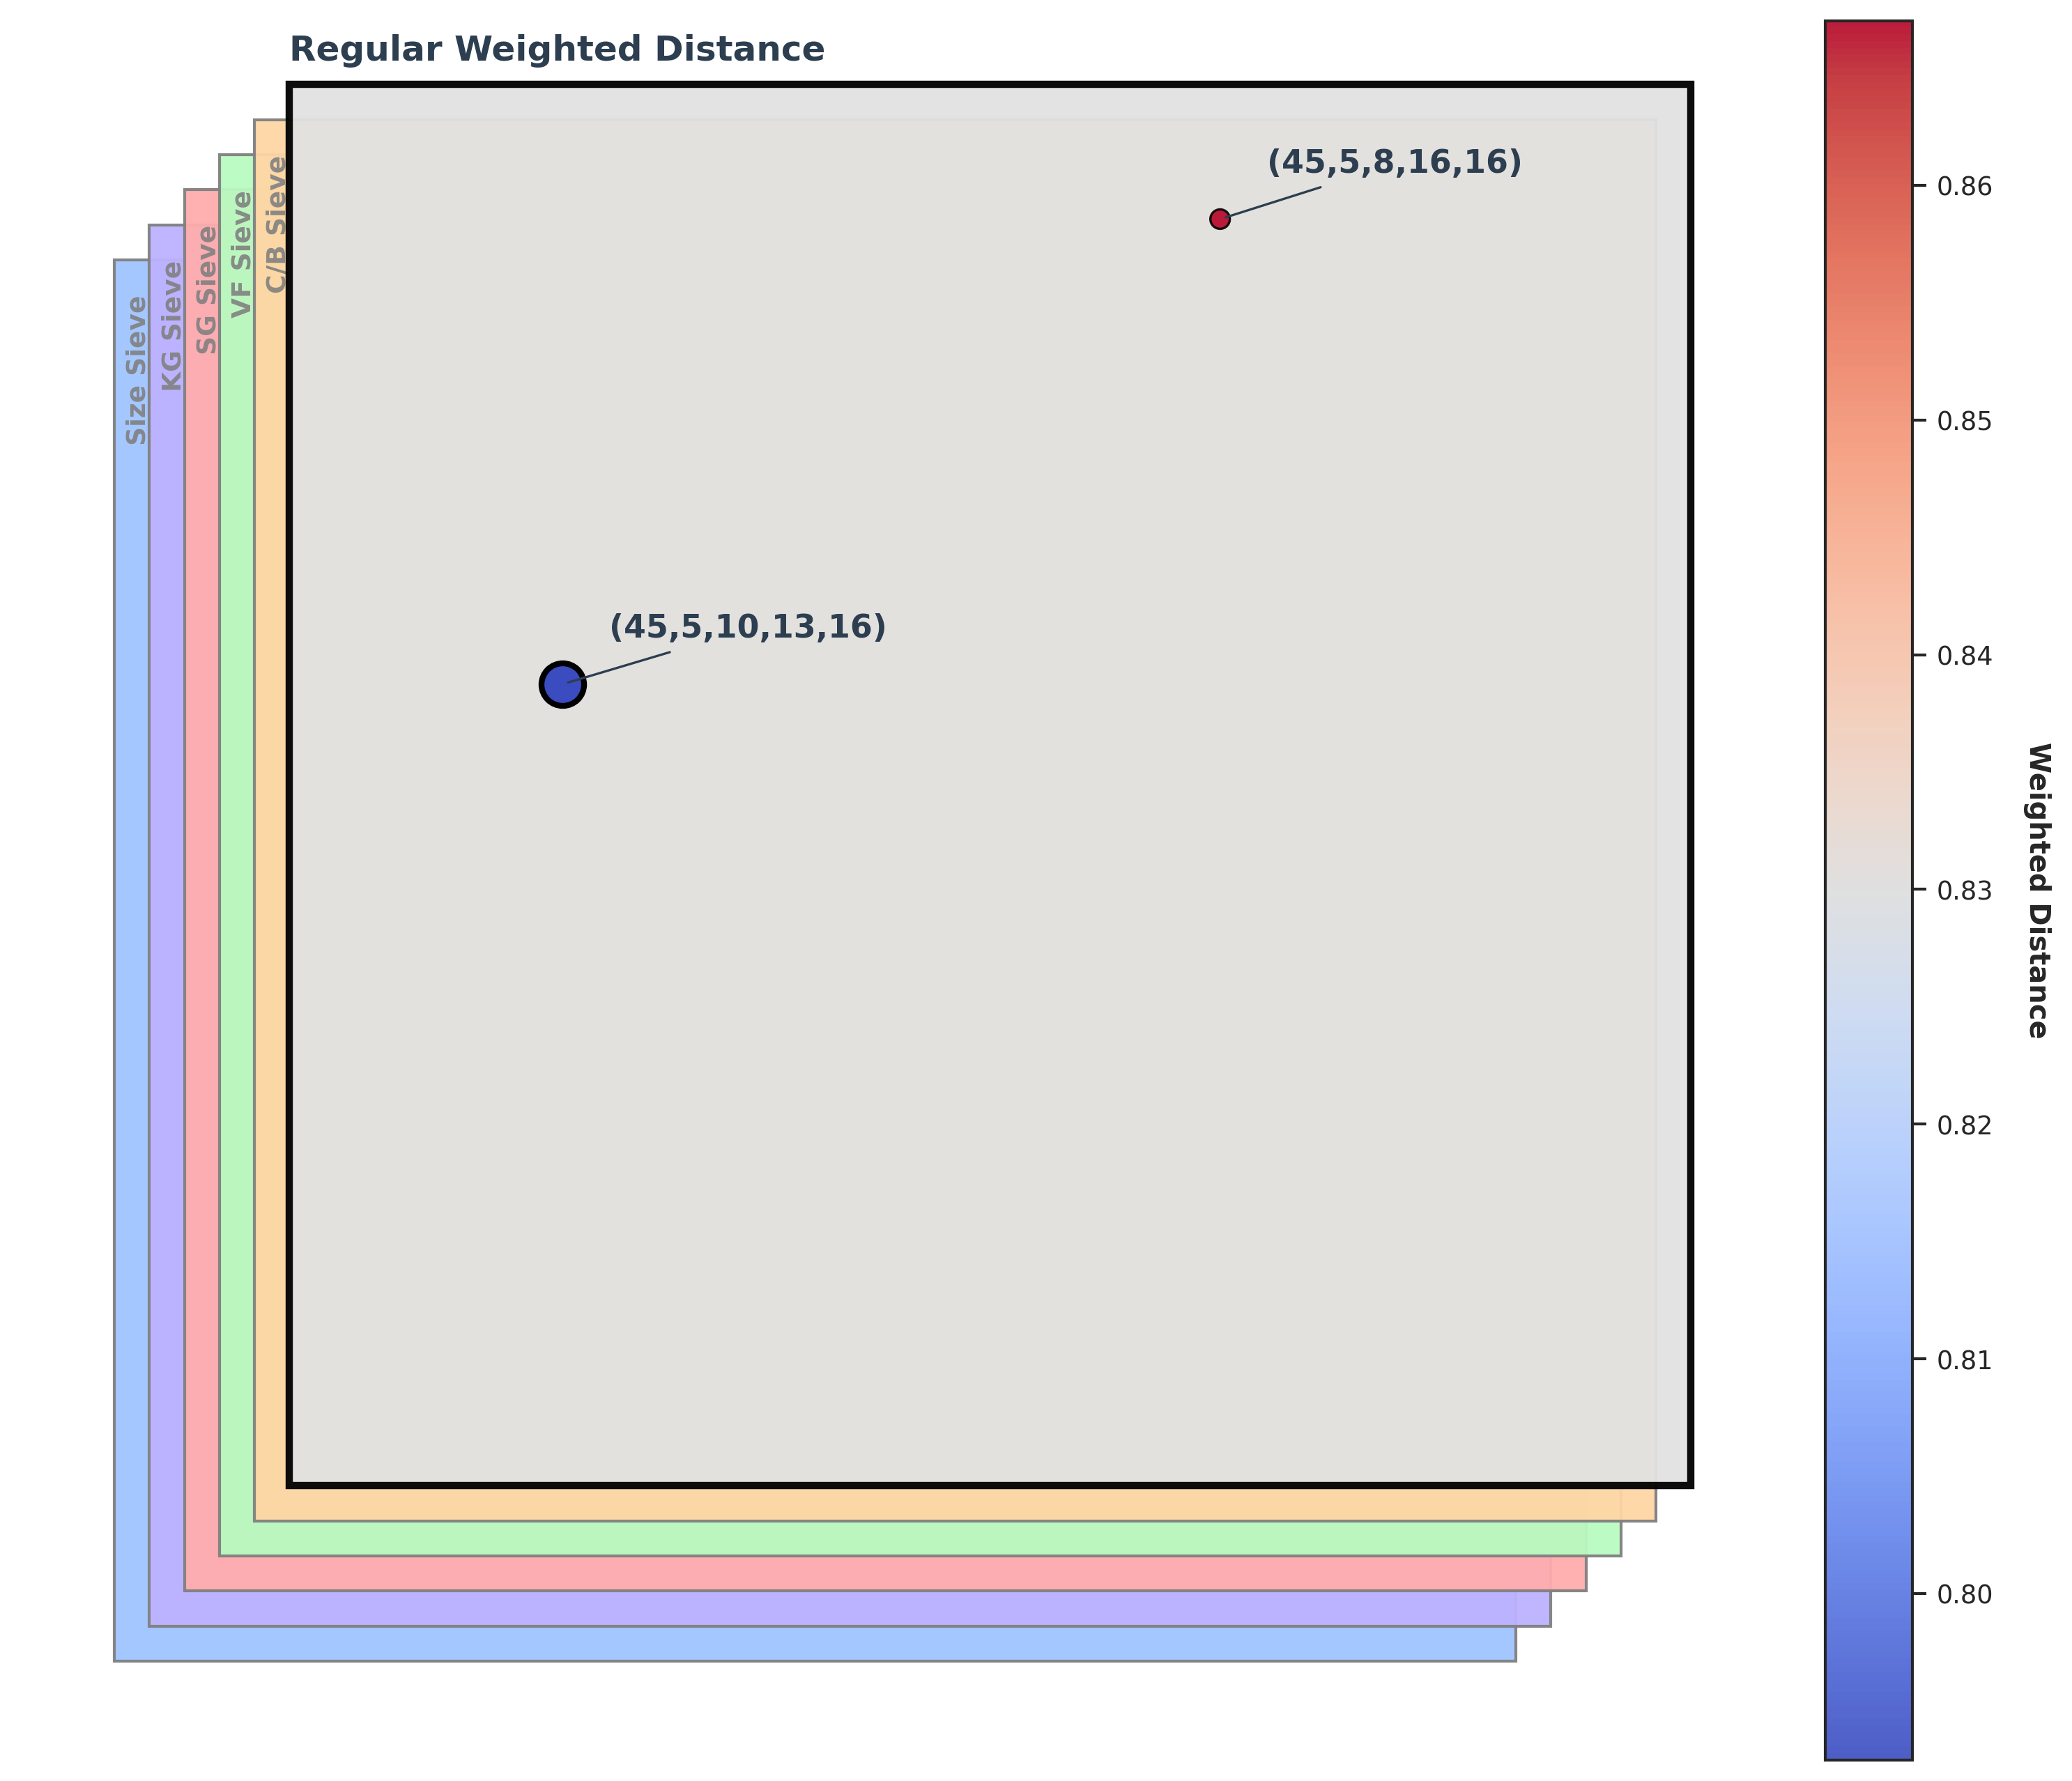
\includegraphics[width=\textwidth]{content/images/ideal_candidate_balanced.png}
        \caption{Balanced Candidate}
        \label{fig:regular-weighted}
    \end{subfigure}
    \hfill
    \begin{subfigure}[b]{0.49\textwidth}
        \centering
        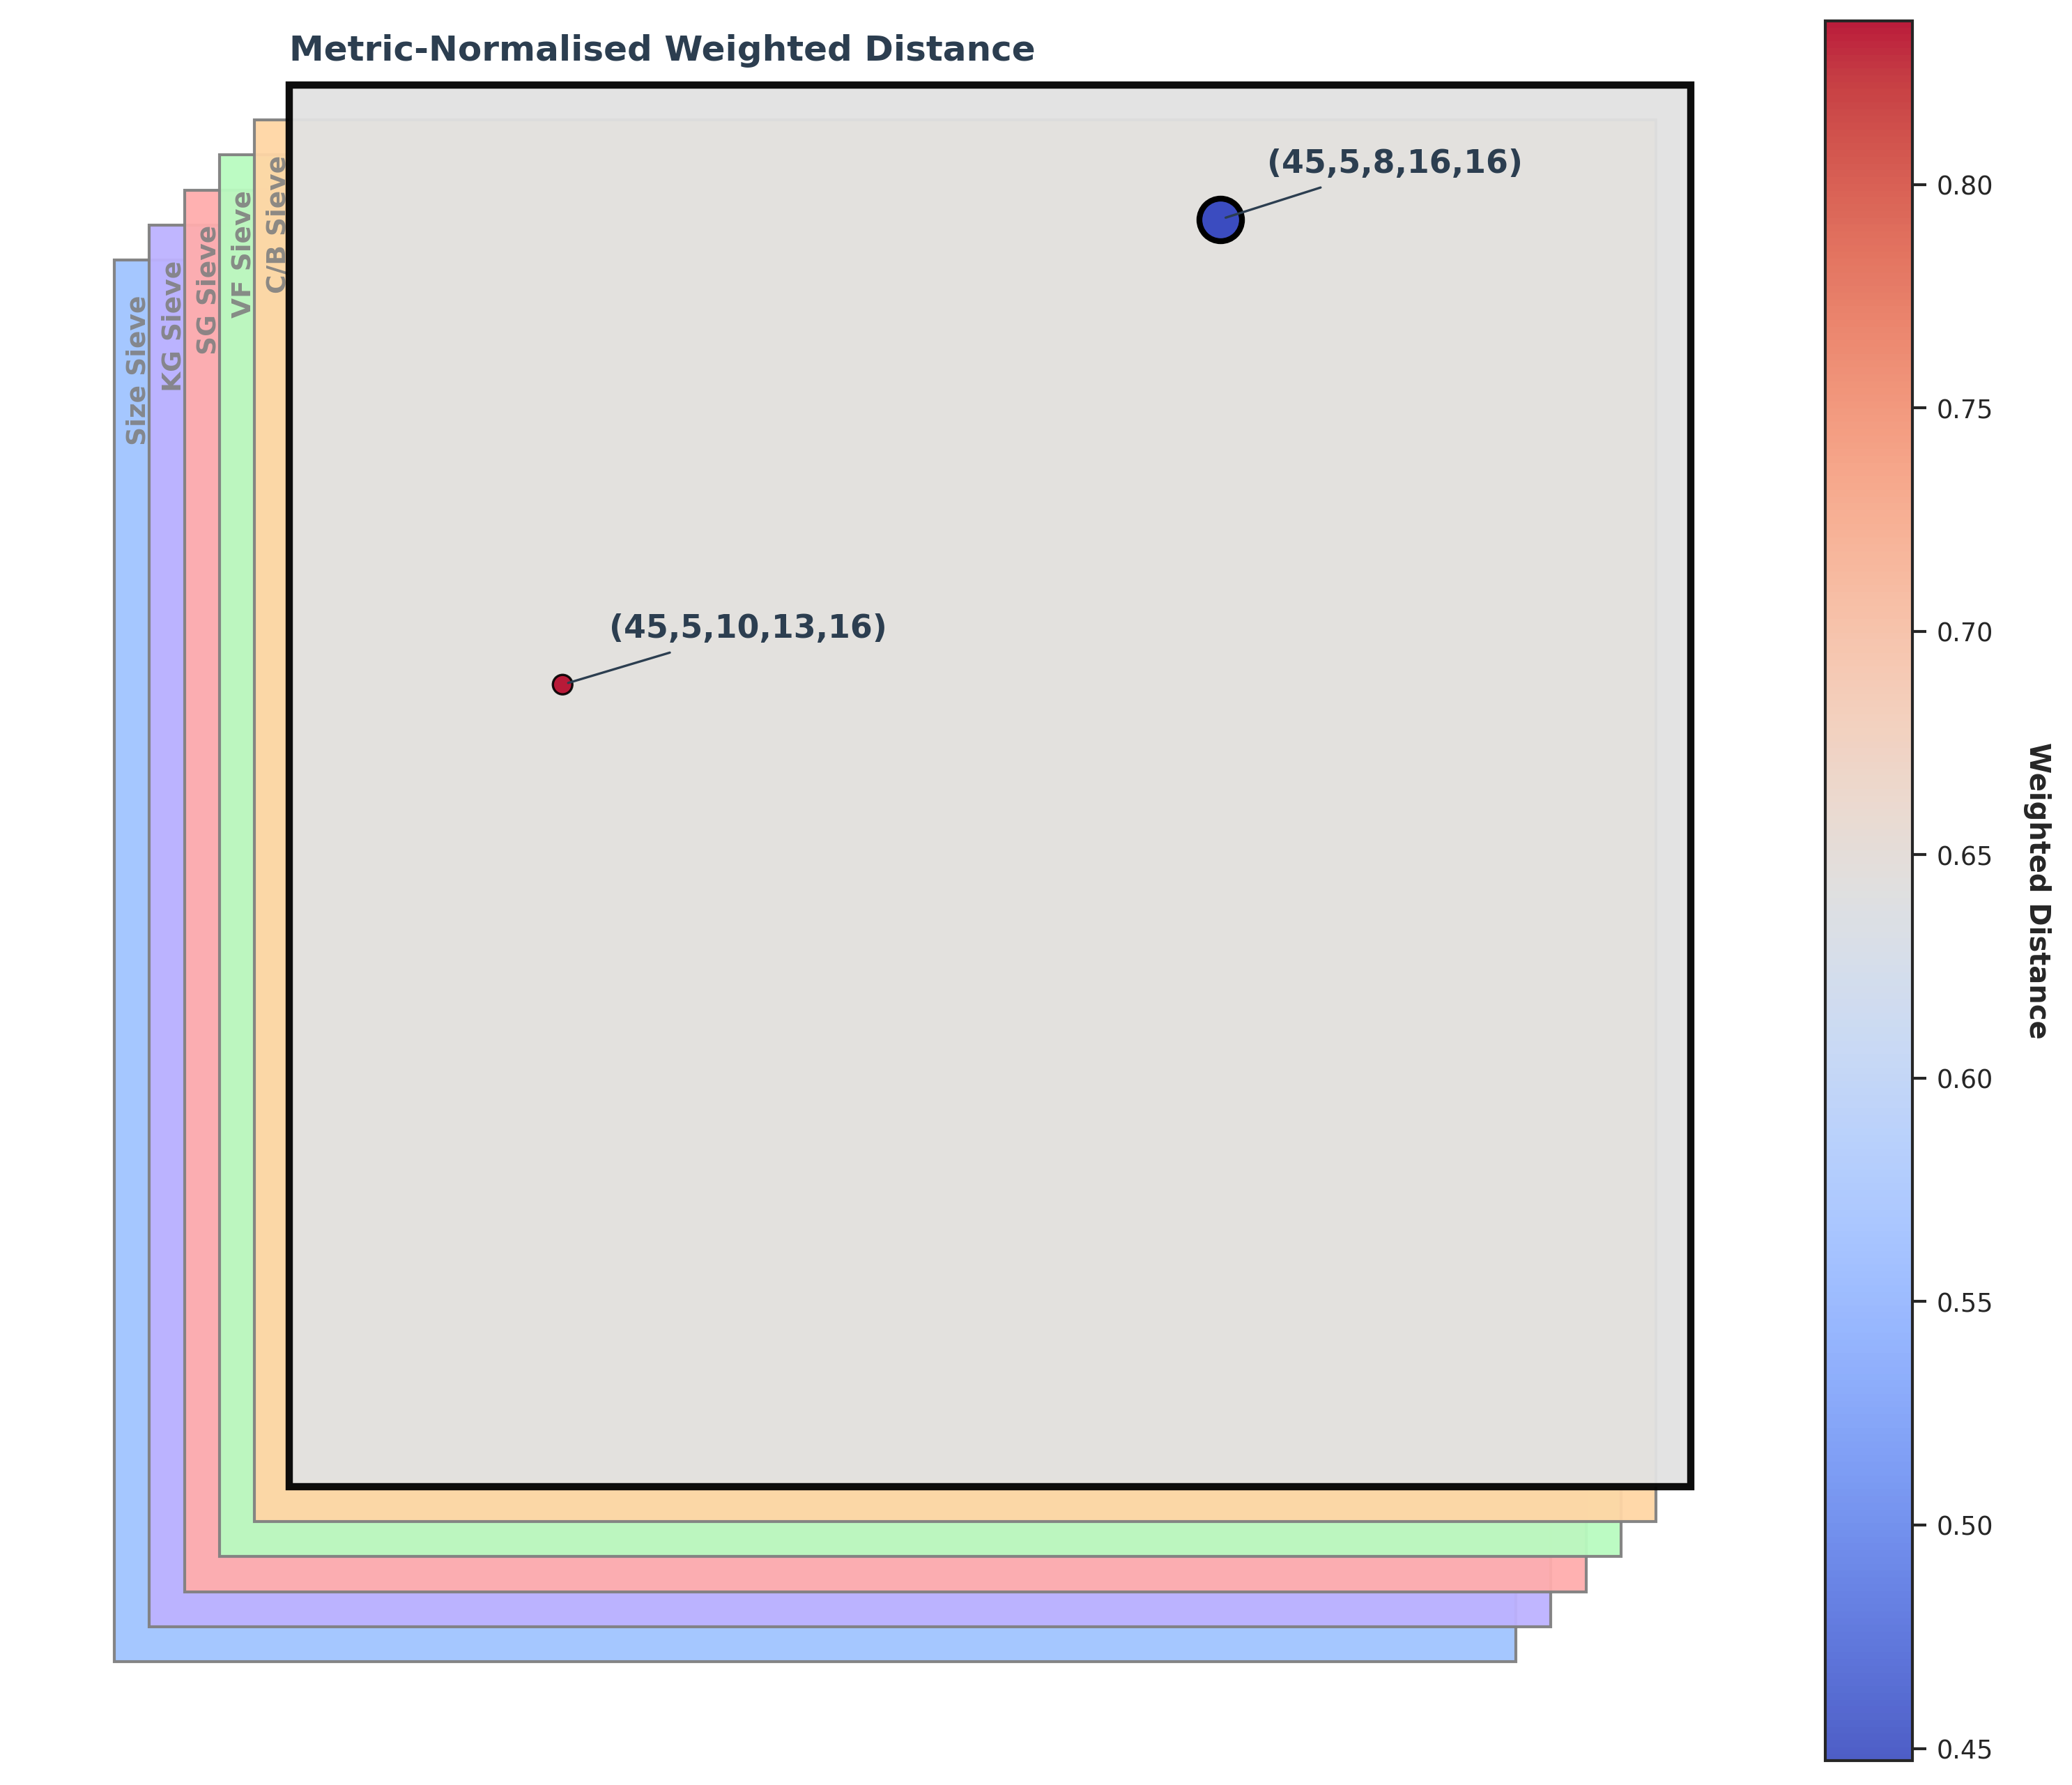
\includegraphics[width=\textwidth]{content/images/ideal_candidate_best.png}
        \caption{The Best Candidate}
        \label{fig:metric-normalised}
    \end{subfigure}
        \caption{The Best Candidate}
\caption{Visualization of Found Candidates After the Search}
\label{fig:ideal_distance_plot}
\end{figure}

The interactive visualization used to produce Figure~\ref{fig:distance_result_comparison}, Figure~\ref{fig:ideal_distance_plot} is publicly available at \url{https://mjthatch.github.io/SPHINCS-Parameters/site/}.

\newpage

\bibliographystyle{plain}
\bibliography{refs}

\end{document}